\documentclass[officiallayout]{tktla}
%\documentclass[officiallayout,a4frame]{tktla}
\usepackage[utf8]{inputenc}
\usepackage{latexsym}
\usepackage{graphicx}
\usepackage[
  backend=biber,
  bibstyle=ieee,
  citestyle=numeric-comp,
    sortlocale=en_US,
    natbib=true,
    url=false, 
    doi=true,
    eprint=false
]{biblatex}
\usepackage{software-biblatex}
\usepackage{pdfpages}
\usepackage[hidelinks]{hyperref}

% Math environments and symbols
\usepackage{amsmath}
\usepackage{amsfonts}

% Lemma environment
%\newtheorem{theorem}{Theorem}[section]
%\newtheorem{lemma}[theorem]{Lemma}

% Independence symbol
\newcommand\indept{\protect\mathpalette{\protect\independenT}{\perp}}
\def\independenT#1#2{\mathrel{\rlap{$#1#2$}\mkern2mu{#1#2}}}

% For thesis papers section
\usepackage{geometry}
\def \dvWHITE{white}
\def \dvBLACK{black}
\def \dvBLUE{blue}
\def \dvGREEN{green}
\def \dvheight{231pt}
% Creates black box with the text given as first parameter in white
\newcommand\note[3] {\marginpar{\vspace{#2}\colorbox{#3}{\parbox[c][\dvheight][t]{34.8pt}{\vspace{0.3cm}\color{white}\centering\Huge{\textbf{#1}}}}}}

% Footnotes without numbering
\let\svthefootnote\thefootnote

\addbibresource{maklin2022.bib}

\title{Probabilistic methods for \\ high-resolution metagenomics}
\author{Tommi Mäklin}
\authorcontact{tommi@maklin.fi\par
  https://maklin.fi/}
\pubtime{June}{2022}
\reportno{0}
\isbnpaperback{000-00-0000-0}
\isbnpdf{000-00-0000-0}
\issn{1238-8645}
\issnonline{2814-4031}
\printhouse{Unigrafia}
\pubpages{7} % --- remember to update this! 
% For monographs, the number of the last page of the list of references
% For article-based theses, the number of the last page of the list of
% references of the preamble part + the total number of the pages of
% the original articles and interleaf pages.
\supervisorlist{Antti Honkela, University of Helsinki, Finland \\ \hspace{8pt} Jukka Corander, University of Helsinki, Finland}
\preexaminera{Ashlee Earl, Broad Institute of MIT and Harvard, USA}
\preexaminerb{Tommi Vatanen, University of Auckland, New Zealand}
\opponent{To be appointed}
\custos{To be appointed}
\generalterms{Algorithms, Experimentation}
\additionalkeywords{genomic epidemiology, plate sweeps, probabilistic modeling, pathogen surveillance, taxonomic profiling, taxonomic binning, metagenomics}
% Computing Reviews 1998 style
%\crcshort{A.0, C.0.0}
%\crclong{
%\item[A.0] Example Category
%\item[C.0.0] Another Example
%}
% Computing Reviews 2012 style
\crclong{
\item Mathematics of computing $\rightarrow$ Probability and statistics $\rightarrow$ Statistical computing
\item Computing applications $\rightarrow$ Biosciences
}

\permissionnotice{
  Doctoral dissertation, to be presented for public examination with 
  the permission of the Faculty of Science of the University of
  Helsinki in \ldots{} on \ldots{} at XX o'clock. Fill in the examination
  venue, date and time into the previous sentence.
}

\newtheorem{theorem}{Theorem}[chapter]
\newenvironment{proof}{\noindent\textbf{Proof.} }{$\Box$}

\begin{document}

\frontmatter

\maketitle

\begin{abstract}
  Metagenomics is the analysis of DNA sequencing data from samples
  obtained directly from the environment and containing several
  different organisms at once. Common tasks in metagenomics are
  taxonomic profiling, where the goal is to identify the organisms
  present in the sample and assign relative abundances to them, and
  taxonomic binning, where the sequencing data from the sample is
  divided into bins that correspond to some sensible taxonomic
  units. In this thesis I introduce methods for performing these two
  tasks at a high-resolution capable of distinguishing between
  lineages of bacterial species. The first of these methods is mSWEEP,
  which solves the profiling task by utilizing a collection of grouped
  bacterial reference sequences, pseudoalignment, and a probabilistic
  model. The second method, mGEMS, builds upon mSWEEP to solve the
  binning task using an assignment rule derived from the fundamentals
  of the probabilistic model used by mSWEEP.

  Both mSWEEP and mGEMS have been developed for application in either
  the traditional whole-genome shotgun metagenomics context, where the
  direct-from-environment samples are analysed, or in the plate sweep
  metagenomics context, where the sample has been plated once on a
  selective medium. While the latter is not metagenomics in the
  traditional sense, this thesis advocates for its use when high depth
  sequencing data is required from some species and the other
  organisms are not of interest. Regardless of the type of
  metagenomics data used, the ultimate goal of both mSWEEP and mGEMS
  is to enable performing standard genomic epidemiological analyses
  directly from data containing several strains of the same bacteria,
  skipping the typically used isolation steps required to separate
  them. Due to the implied cost-savings from reducing the number of
  cultures that need to be performed as well as the better capture of
  variation in the samples through using metagenomics data, mSWEEP and
  mGEMS hopefully enable performing entirely novel types of analyses
  in the field of genomic epidemiology.

\end{abstract}

\begin{acknowledgements}
  acknowledgements
   \begin{flushright}
  place\\
  author
  \end{flushright}
\end{acknowledgements}

\tableofcontents

\mainmatter

\chapter{Introduction}

Public health research focusing on bacterial pathogens has been
transformed by analysis of the contents of bacterial genomes obtained
by whole-genome sequencing (WGS) during the past few decades
\citep{armstrong2019pathogen}. In this time frame, the price of
sequencing has decreased tremendously \citep{dnaseqcost,
  goodwin2016coming}, enabling adoption of sequencing as a standard
tool in the infectious diseases and genomic epidemiology toolkits
\citep{tang2017infection, grad2014epidemiologic, kwong2015whole}. Many
of the standard analyses in these fields require data from pure
bacterial cultures, created by isolating a bacterium on its own plate
from an initial mixed culture, which often contain several distinct
bacteria and other micro-organisms. Isolating all of these presents
substantial economical barriers to more widespread adoption of WGS as
a routine tool since the cost and turnaround time of the library
preparation and DNA extraction steps, performed once per each isolated
organism, are approaching the price of sequencing itself \citep{rossen2018practical}.

Whole-genome shotgun metagenomics, where DNA is extracted and
sequenced directly from the original environmental sample, presents a
potential cost-effective alternative to the isolate sequencing
approach. Contrary to isolate sequencing, WGS metagenomics requires
only a single library preparation and DNA extraction step and no
cultivation steps since the sample is sequenced directly. However,
direct sequencing may require significantly higher sequencing depths
due to presence of host DNA \citep{pereira2019impact,
  mcardle2020sensitivity} and contamination
\citep{mcardle2020sensitivity, salter2014reagent}. Due to these
factors, WGS metagenomics can be difficult to apply when only a subset
of the diversity is targeted but the planned analyses require high
sequencing depth data, which is the typical setting in genomic
epidemiological studies.

Genomic epidemiology is the study of the spread and transmission of
bacterial pathogens based on WGS data. Sequencing the genomes of
bacterial pathogens during an outbreak allows for comparing
accumulated mutations in their genomes \citep{tang2017infection},
elucidating their short-term evolutionary history and enabling case
linking when combined with appropriate metadata
\citep{grad2014epidemiologic, hill2021progress}. Similarly, long-term
routine surveillance aids in hastening the detection of outbreaks
\citep{eyre2012pilot, gardy2018towards}, identifying potential
high-risk clones \citep{aanensen2016whole}, or reservoirs for
antimicrobial resistance \citep{weingarten2018genomic,
  coipan2020genomic}. Many of these analyses require assembling the
genomes of the bacteria from the sequencing reads which has led to
dominance of the isolate sequencing approach and a lack of studies
attempting to solve the problems with metagenomics.

When choosing between WGS metagenomics and isolate sequencing, a
middle-ground can be found plate sweep metagenomics
\cite{maklin_high-resolution_2021} \textemdash{ } sometimes also called
limited-diversity metagenomics \citep{cocker_drivers_2022}. In this
approach the initial culture from an environmental sample is swept
and sequenced in its entirety rather than preparing several isolate
cultures from it. Since selective culture media are available for many
clinically relevant bacteria \citep{lagier2015current}, plate sweep
metagenomics simultaneously both reduces the number of library
preparation \& DNA extraction steps by using only a single culture,
and solves the host DNA overabundance \& sequencing depth issues in
WGS metagenomics through selective media enrichment. Incorporating an
enrichment step has also been found to increase the sensitivity to
low-abundance organisms that might be missed in direct sequencing
\citep{whelan2020culture}.

While both plate sweep metagenomics and WGS metagenomics have
technically been possible for many years with the latter appearing
around 2004 \citep{tyson2004community, venter2004environmental}, the
development of computational methods has largely focused on analysing
sequencing reads from a single organism at a time. Although many
methods for analysis of metagenomic data at the species-level have
been developed \citep{breitwieser2019review}, these do not typically
perform well when applied to data containing strain-level variation
\citep{sczyrba2017critical}. Methods diverging from the traditional
relative abundance estimation (taxonomic profiling)
\citep{truong2017microbial} or metagenomic sequence read demixing
(taxonomic binning) \citep{van2022strainge} context do successfully
tackle strain-level variation but do not easily translate to replacing
assembly-based analyses such as SNP calling or phylogenetic inference.

In this thesis I present two computational methods that enable
taxonomic profiling and taxonomic binning from either WGS metagenomic
or plate sweep metagenomic short-read sequencing data. While the plate
sweep metagenomics approach was required by both methods during their
initial publication, I also demonstrate that they perform reliably
when applied to WGS metagenomics data. Using either of the two
approaches to reduce the costs associated with data collection, the
methods presented here enable performing routine genomic
epidemiological analyses when significant strain-level is present in
the collected sequencing data.

The first of the two methods, called mSWEEP, consists of a
probabilistic model for estimating the relative abundances of lineages
of a bacterial species in a set of sequencing reads
\citep{maklin_high-resolution_2021}. mSWEEP leverages pseudoalignment
\citep{bray2016near} of the reads against a set of reference sequences
that have been grouped together into lineages and outputs estimates of
the lineage-level abundances. The second method, mGEMS, processes the
output from mSWEEP to construct an assignment rule for assigning each
read to one or more bins corresponding to a reference lineage
\citep{maklin_bacterial_2021}. Both methods explicitly account for the
fundamental characteristic of within-species sequencing data where
each read can and often does belong to several lineages of the same
species at the same time. The combination of mSWEEP and mGEMS enables
effective computational quantification of metagenomic data at a high
resolution within the species, and enables downstream processing of
mixed samples with results comparable to using isolate data.

Even though both mSWEEP and mGEMS were originally designed with
applications in plate sweep metagenomics in mind, this thesis includes
a third article \citep{maklin_strong_2022} that demonstrates
applicability of both methods to WGS metagenomics data. In the third
article, we have analysed WGS metagenomics data from babies born in
the UK collected during their neonatal period
\citep{shao2019stunted}. Results from this data show strong
competition between bacterial species and strains during the initial
colonization of the newborn gut microbiome. More importantly from a
methods perspective, this analysis shows that mSWEEP and mGEMS provide
(so-far) completely unprecedented levels of resolution in analysis of
metagenomic sequencing data.

Together the three articles in this thesis represent foundational
methodological steps in both opening up high-resolution exploration of
bacterial diversity as well as making such analyses more accessible to
resource-constrained laboratories.

\section{Three approaches to sequencing bacterial DNA}
\label{three-approaches-to-metagenomics}

%- Something about sequeuncing reads and sequence assembly? 16S sequencing?

Preparing bacterial DNA for sequencing is often done after a
culture step that enriches the number of bacterial cells. Culturing
is performed by plating a sample and inoculating it for a period of
time that allows the bacteria to multiply
\citep{sanders2012aseptic}. After inoculation, visible colonies may be
isolated and further propagated on their own plates
\citep{sanders2012aseptic}, or the whole plate may be prepared for DNA
extraction to produce plate sweep metagenomic data. Alternatively, in
WGS metagenomics, the whole culture procedure is skipped, and DNA is
extracted directly from the sample with the extract procedure
depending on the sample type \citep{bachmann2018advances}. When it
comes to the end-result \textemdash{ } the sequencing reads \textemdash{ }
all three approaches have their own characteristics that affect the
available downstream analyses.

% TODO read and cite
% https://link.springer.com/article/10.1007/s00253-018-9209-9 and
% https://www.annualreviews.org/doi/10.1146/annurev-pathmechdis-012418-012751

WGS metagenomics, where all or most of the DNA in a sample is
extracted (Figure \ref{fig:microbiome-sampling-methods}a), has emerged
as a tool for analysing the full breadth of variety in various
microbiomes (TODO citations, at least babybiome paper plus
others). Exploring this diversity comes at a price, however, since the
produced sequencing reads are split across the numerous organisms
possibly present, resulting in a need to sequence the sample more
deeply to analyse the less abundant organisms (TODO
citations). Combined with other issues related to host DNA abundance
(TODO citations) and a lack of bioinformatics resources (TODO
citations), the shortcomings of WGS metagenomics have so-far prevented
its widespread adoption as a standard tool (TODO citations).

Plate sweep metagenomics proposes a middle-ground between the direct
sequencing of WGS metagenomics and isolate studies by incorporating a
single culture step \citep{maklin_high-resolution_2021}. In this
approach, the sample is cultured on an appropriate selective media and
the entire complexity of the plate is sequenced after a suitable
inoculation period (Figure
\ref{fig:microbiome-sampling-methods}b). The inclusion of a culturing
step allows for generating large numbers of sequencing reads from the
bacteria that thrive in the chosen media, circumventing both the
sequencing depth and host DNA issues in WGS metagenomics while
improving the sensitivity to bacteria found in low abundance in the
original sample (TODO citations, cystic fibrosis study + gerry's
study? + see if there are others). Furthermore, focusing the
sequencing efforts on the relevant bacteria enables application of
bioinformatics tools that require a high sequencing depth provided
that the reads from different organisms can be computationally
separated. Developing a tool to solve the aforementioned deconvolution
problem is one of the key contributions of this thesis.

\noindent\let\thefootnote\relax\footnote{Figure source: Adapted from \cite{praveera_fenugreek-sprouts} and \cite{niaid_escherichia-coli}. Released under the \href{https://creativecommons.org/licenses/by-sa/4.0}{CC BY-SA 4.0 license}.}
\addtocounter{footnote}{-1}\let\thefootnote\svthefootnote
\begin{figure}[!ht]
  \label{fig:microbiome-sampling-methods}
    \centering
    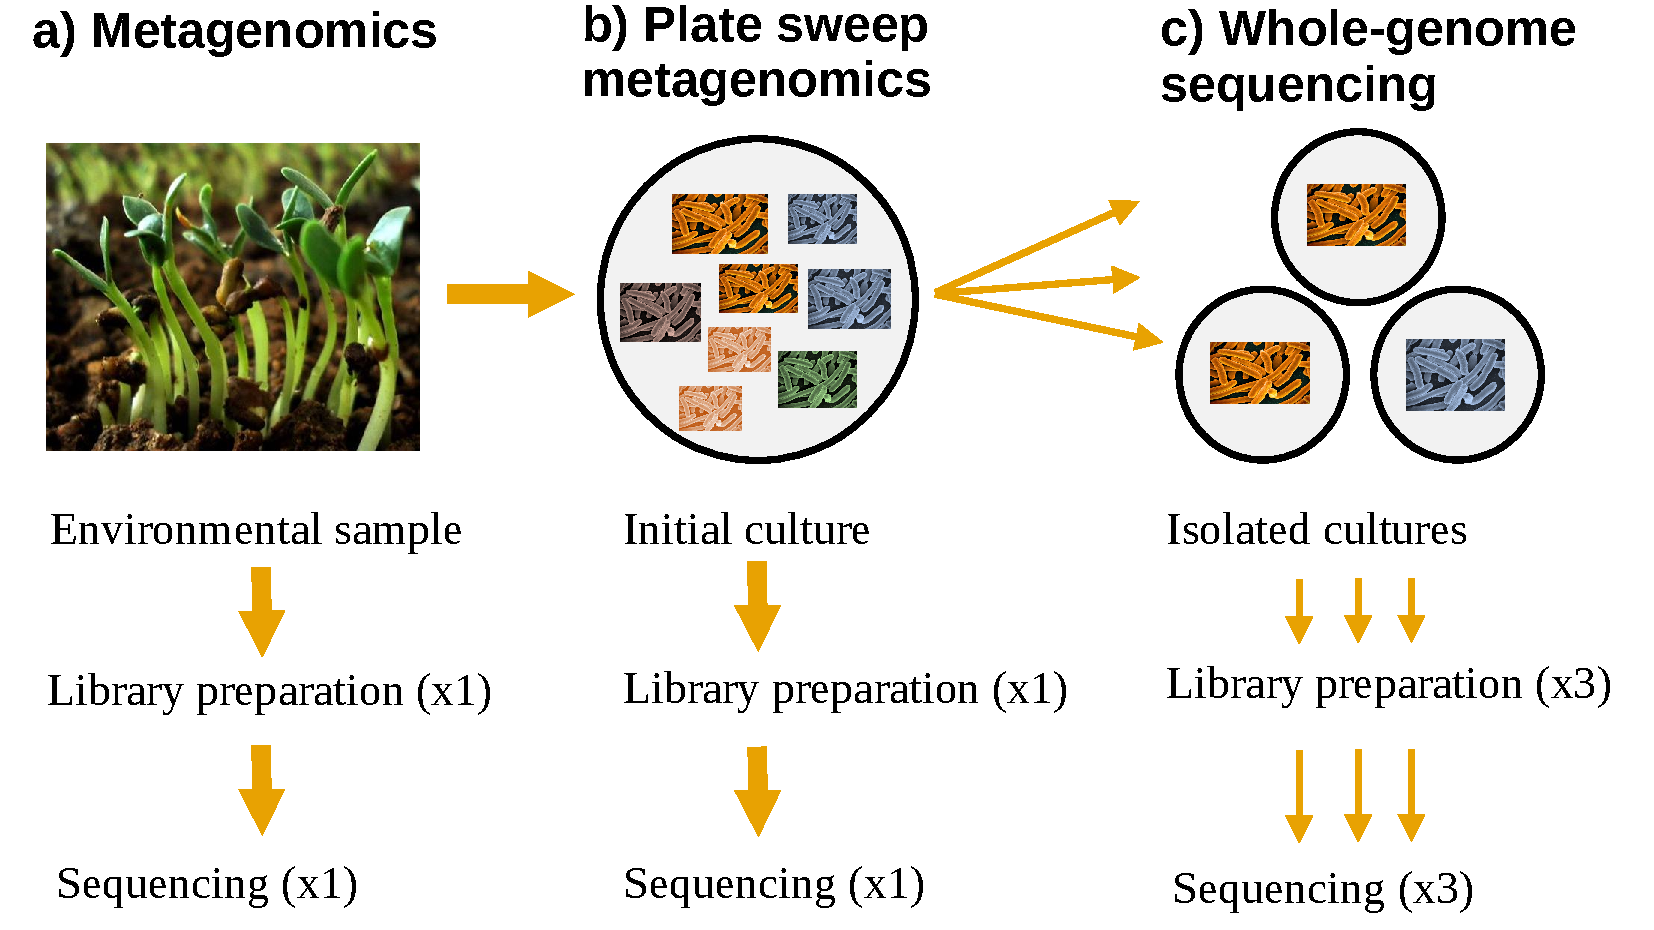
\includegraphics[width=\textwidth,keepaspectratio]{img/sampling/microbiome_sampling_methods.pdf}
    \caption{Different approaches to sequencing bacterial DNA. Panel
      \textbf{a)} depicts the WGS metagenomics approach, where
      sequence data is collected directly from the sample. Panel
      \textbf{b)} depicts the plate sweep metagenomics approach, where
      the sample is plated on a selective medium and DNA is sequenced
      from the whole plate after an inoculation period. Panel
      \textbf{c)} depicts the whole-genome sequencing approach, where
      a subset of visible colonies on the inoculated culture are
      extracted and transferred to their own plates, inoculated again,
      and then prepared for sequencing.}
\end{figure}

% (TODO citations for this paragraph? common knowledge but could try
% to find some manual explaining the colony picks.
In the third approach, whole-genome sequencing of isolates (Figure
\ref{fig:microbiome-sampling-methods}c), visible colonies from the
initial culture are picked and transferred to new plates. After
letting the transferred colonies inoculate, the resulting culture will
consist only of the descendants of the original colony, allowing for
massive numbers of sequencing reads to be generated from the isolated
organisms. Since visible colonies on the initial culture are typically
assumed to contain clones of the same organism, this approach
effectively gets rid of all the variation found in both the sample and
the initial culture. While the whole-genome sequencing approach is
excellent for generating high-coverage and high-quality data from a
single bacterial strain, in practice the number of colonies that can
be isolated is often constrained by laboratory resources and nearly
always restricted to rapidly growing colony-forming phenotypes.

In genomic epidemiological analyses, the whole-genome sequencing
approach has been dominant due to the ability to produce highly
accurate genomic data (TODO citation). Producing the same results
using WGS (or plate sweep) metagenomics has some obvious benefits in
both increasing the number of samples that can be processed as well as
in capturing more of the diversity in the samples, but the existing
metagenome-analysis tools have not been able to reach the required
level of resolution (TODO citation). In this thesis I tackle the issue
and present methodological advances that may finally open up more
widespread use of metagenomic sequencing data in genomic epidemiology.

\section{Analysing metagenomic sequence data}

\textbf{- Need a picture of the different approaches.}

Metagenomic sequencing data analysis presents several challenges to
bioinformaticians (TODO citations). Firstly, the increased diversity
of species requires much larger computational resources to analyse
(TODO citation). Secondly, the possible presence of strain-level
variation complicates analyses that attempt to separate the reads to
distinct taxonomic units because the differences between strains
within a species are often minimal (TODO citation). Subsequently, the
majority of methods development has focused on operating with the
assumption that only a single strain from each species is present in
the same sample (TODO citation, review by florian breitweiser?). In
this section I will briefly cover some of the previous approaches and
describe how mSWEEP and mGEMS fit into the metagenomics toolkit.

% TODO cite some appropriate reviews, check mGEMS paper
One of the more commonly used tools for analysing WGS metagenomics
data are metagenome assemblers. Similarly to genome assemblers,
metagenome assemblers aim to produce a set of contigs that correspond
overlapping sequencing reads. Since reads from metagenomic sequencing
contain several organisms, metagenome assemblers are often paired with
metagenome binners that attempt to assign the metagenome-assembled
contigs to bins that correspond to a taxonomic unit. These units are
typically assumed distinct enough that they are not mistaken for
sequencing error or minor genetic variation. When the assumption is
fulfilled, metagenome assemblers produce contigs that are adequately
accurate for several types of analyses, and have subsequently been
adopted among the standard tools in a variety of microbiome studies
(TODO citations).

% TODO cite some appropriate reviews, check mGEMS paper
Metagenome binners are closely related to another type of analysis,
where the aim is to assign (relative) abundances to the taxonomic
units that were identified in the sequencing reads, called taxonomic
profiling. These two approaches sometimes go hand-in-hand since the
abundance of a taxonomic unit can naively be defined as the number of
contigs assigned to the unit. When the units are closely related
species or strains, more sophisticated methods are necessary since the
contigs may plausibly belong to several taxa, which has led to the
development of dedicated taxonomic profilers that do not attempt to
bin the contigs or sequencing reads (TODO cite metaphlan, msweep,
others).

% TODO citations
Recently, a third category of methods attempting to track the
presence/absence of a specific strain of bacteria across several
samples has emerged (TODO cite strainge, strianphlan, midas?). Methods
in this category aim to infer similarity and shared strains and
provide an attractive tool for transmission analysis when the genome
assemblies of the individual strains are not required or cannot be
assembled due to the sequencing depth. Ideally, the tools for tracking
strains would be combined with those for extracting the contig or read
bins, together enabling both a wide analysis covering all samples and
strains and a focused analysis of the strains that are found in high enough
abundance to assemble their genomes.

% TODO citations? or is this original content
All of the above can be further divided into reference-based methods
that leverage reference data in their analysis, and reference-free
methods that perform the analysis solely based on the sequencing
reads. While reference-free methods are able to handle data containing
previously unknown bacteria that do not have any available genome
assemblies, reference-based methods provide an easily interpretable
context for the results and typically reach a higher resolution (TODO
citation). If detailed quantification is only required for some subset
of organisms in the sample, reference-based methods frequently also
provide means to filter out the reads belonging to the uninteresting
organisms.

The strain-level methods from this thesis take the reference-based
approach and specifically leverage bespoke reference
collections. Tailoring the reference genome assemblies to fit the
presumed contents of the samples allows both mSWEEP and mGEMS to
perform at a resolution that is mainly limited by the quality and
variety of the available assemblies. Contrary to many existing
reference-based methods, mSWEEP and mGEMS do not attempt
identification of the individual reference sequences, but rather
incorporate a clustering of the reference assemblies within a species
to biologically sensible lineages. Since the lineage-level differences
are generally more pronounced, the identification task at this level
becomes significantly easier (cite BIB paper) and additionally allows
for handling cases where the sequencing reads originate from an
unknown sequence which belongs to a known reference lineage. Trading
the ability to imprecisely identify the exact sequence to precisely
identifying the lineage it belongs to is especially useful in clinical
settings, where the diversity of potential pathogenic bacteria has
been thoroughly studied using whole-genome sequencing (TODO citation)
and the clinically relevant lineages are often well-known.

\section{Using metagenomics data in genomic epidemiology}

\textbf{Figure about genomic epidemiology analyses}

Aside metagenomics tools, the second significant aspect of this thesis
has to do with their application in genomic epidemiology, where the
goal is to trace the transmission of pathogenic bacteria using genomic
sequence data. Genome-informed analyses have in recent years greatly
expanded the ability of researchers to investigate outbreaks, identify
epidemiologically relevant genetic elements, and detect emerging
public health concerns (TODO citations). Due to the high level of
accuracy required, these analyses have been performed using isolate
WGS data, which has a relatively high economical cost and slow
turnaround time (TODO citations, one of the already cited papers),
rendering the research more reactive in nature. One of the goals of
mSWEEP and mGEMS is to enable partially replacing the use of isolate
data with metagenomics data, decreasing both the cost and turnaround
time of the existing genomic epidemiology pipelines.

In addition to the improving both cost- and time-effectiveness,
incorporating some kind of metagenomics data into genomic epidemiology
presents some obviously attractive advantages in increasing the
sensitivity to genetic diversity that might be obscured by the use of
isolate data in routine surveillance (TODO citation?). As an example,
a recent study into within-host diversity of the common respiratory
pathogen \textit{Streptococcus pneumoniae} utilized an analogue of
plate sweep metagenomics and found low-frequency co-colonization of
epidemic serotypes alongside known carriage serotypes
\citep{tonkin-hill_pneumococcal_2022}. This finding helped explain the
previously unknown source of the epidemic serotypes in outbreaks of
disease, which could not be fully explained by isolate sequencing
data. Since naturally occurring variation is common in many species of
clinical interest (TODO citations), similar findings in other fields
are likely with more widespread use of metagenomics data.

% TODO this *really* needs citations
Another related aspect in favour of using more metagenomics-oriented
approaches arises from simple practicality: sequencing several
organisms at once is simply easier than performing the several steps
required to isolate an organism for DNA extraction. Direct sequencing
of the samples combined with nearly equally accurate analyses should,
in principle, make implementing routine surveillance significantly
more accessible to locations and laboratories lacking in funding and
resources. This in turn combined with data sharing practices across
borders has the potential to vastly increase the capabilities of
proactive surveillance. Furthermore, sequencing the whole sample and
publicly archiving the reads has the benefit of preserving the full
variety of organisms in the sample and making it available for future
analyses with different goals from the original studies.

In conclusion, the field of genomic epidemiology that was established
with the spread of WGS sequencing in the early 2010's can be seen as
entering a transformative period with the price of data generation
decreasing and more powerful computation tools becoming available. The
development of methods such as mSWEEP and mGEMS will, hopefully,
further speed up this transformation and enable entirely novel types
of analyses and discoveries through the inclusion of metagenomic data.

\section{Contributions}

This thesis comprises three publications covering both mSWEEP
\citep{maklin_high-resolution_2021} and mGEMS
\citep{maklin_bacterial_2021} as well as a third article demonstrating
their application to whole-genome shotgun metagenomic sequencing data
\citep{maklin_strong_2022}. The first two publications are accompanied
by software implementations \citep{maklin_mSWEEP, maklin_mGEMS}. The
third article is more applied in nature, exploring in more detail the
types of analyses enabled by the first two papers.

\subsection*{Paper I \textemdash{ } High-resolution sweep metagenomics using fast probabilistic inference}
By \underline{Tommi Mäklin}, Teemu Kallonen, Sophia David, Christine J
Boinett, Ben Pascoe, Guillaume Méric, David M Aanensen, Edward J Feil,
Stephen Baker, Julian Parkhill, Samuel K Sheppard, Jukka Corander, and
Antti Honkela. Published in \textit{Wellcome Open Research} (2021),
5:14, doi: 10.12688/wellcomeopenres.15639.2.

In the first paper \citep{maklin_high-resolution_2021}, we presented
and benchmarked the mSWEEP method for taxonomic profiling of
sequencing data containing multiple strains from the same bacterial
species. My contributions included conceptualization of the study,
formal analysis and investigation of the data, developing the
methodology and software implementations, validation and visualization
of the results, and writing \& editing both the original draft and the
revised manuscript.

Software implementation of the ideas presented in Paper I is
available from GitHub at
\href{https://github.com/PROBIC/mSWEEP}{PROBIC/mSWEEP} (latest
version). The latest version at the time of writing is archived and
available in Zenodo \citep{maklin_mSWEEP}.

\subsection*{Paper II \textemdash{ } Bacterial genomic epidemiology with mixed samples}
By \underline{Tommi Mäklin}, Teemu Kallonen, Jarno Alanko, Ørjan
Samuelsen, Kristin Hegstad, Veli Mäkinen, Jukka Corander, Eva Heinz,
and Antti Honkela. Published in \textit{Microbial Genomics} (2021)
7.11, doi: 10.1099/mgen.0.000691.

The second paper \citep{maklin_bacterial_2021} continued to build upon
mSWEEP by developing an algorithm for binning sequencing reads at
lineage-level of mSWEEP. This approach and the accompanying software
implementation are both mGEMS. I contributed to the second paper by
taking part in conceiving the study, developing the mGEMS pipeline, in
designing both the synthetic and the \textit{in vitro} experiments,
developing the mGEMS assignment algorithm, running the experiments,
creating the visualizations, interpreting the results, and in writing
\& editing the main manuscript and the final published version

Software implementation of the ideas presented in Paper II is
available from GitHub at
\href{https://github.com/PROBIC/mGEMS}{PROBIC/mGEMS} (latest version).
The latest version at the time of writing is archived and available in
Zenodo \citep{maklin_mGEMS}.

\subsection*{Paper III \textemdash{ } Strong pathogen competition in neonatal gut colonization}
By \underline{Tommi Mäklin}, Harry Thorpe, Anna Pöntinen, Rebecca
Gladstone, Yan Shao, Maiju Pesonen, Alan McNally, Ørjan Samuelsen, Pål
Johnsen, Trevor Lawley, Antti Honkela, and Jukka Corander. Awaiting
peer-review; available from \textit{bioRxiv} (2022), doi:
XXX.XX/XXX.XXX.XXX.

The third paper \citep{maklin_strong_2022} provides an example of
applying mSWEEP and mGEMS to whole-genome shotgun metagenomics
sequencing data and explores the dynamics of pathogen competition and
colonization in the gut microbiome of babies in their first three
weeks of life. My contributions to this paper include running the
mSWEEP/mGEMS pipeline on all data used in the paper, updating the
reference databases for the investigated species, performing the
analysis of the mSWEEP/mGEMS results for the samples containing
\textit{E. coli}, and aiding the coauthors in analysing the other
species. I additionally contributed to creating the visualisations,
interpreting the results, and naturally to writing the article.

\section{Structure}

The rest of the thesis is structured into three chapters that describe
the contents of the three included papers and how they contribute to
the topics presented in the introduction chapter. The first of the
three chapters describes the basic ideas behind the mSWEEP and mGEMS
methods and provides historical context for the parts of the methods
that have their origins within analysis of RNA sequencing data. The
second chapter describes the experimental results from the three
papers in more detail, focusing more on the applied part rather than
the theoretical foundations. The third chapter is more speculative in
nature, covering both the demonstrated applications from the papers as
well as exploring potential future avenues for use of the developed
methods. The three chapters are followed by a concluding chapter
followed by reprints of the three included original research papers.

\chapter{Mixture modeling of sequence data}

Mixture models are a family of probabilistic models which model
sampling from an overall population as a mixture of sampling from
several distinct subpopulations. Each subpopulation is typically
assumed to have its own distribution, which can be from the same or a
different distribution family, and mixing parameters that determine
the percentages of data each subpopulation contributes to the overall
population.

In sequencing data analysis, a key area of application for mixture
models has been in RNA-Seq, where identifying the expression levels
(relative contributions) of protein isoforms in some set of RNA
sequencing reads is one of the main problems
\citep{garber2011computational, wang2009rna}. Specifically, mixture
models are useful in cases where the sequencing reads do not uniquely
identify the isoform but could plausibly be the product of several
genes. This is in contrast to the microarray technology that preceded
RNA-Seq, where the technology itself allows for unique identification
of the expressed gene and applications of probabilistic models focused
more on obtaining uncertainty estimates (TODO citation).

The ability of mixture models to differentiate between expression of
genes with similar nucleotide contents makes them ideal for analysis
of short-read sequencing data from bacterial strains. Since the
strains within a species typically share a large percentage of their
genome (although the exact values vary greatly by species TODO
citation), sequencing reads from one will match with a large number of
genomes from the same species. Indeed, the models from RNA-Seq have
been adapted almost directly to identify bacterial strains from
sequencing data \citep{sankar2016bayesian} with great effect but not
without some caveats related to more general applicability across
different bacterial species. The work in this thesis extends the
previous work in the field \citep{sankar2016bayesian} by introducing a
more general formulation of the model that generalizes well to
arbitrary bacterial species and allows for assigning sequencing reads
to the bacterial strains in addition to identifying their relative
contributions in a set of sequencing reads.

\section{mSWEEP and mGEMS}

The mSWEEP method is a tool for estimating the relative abundances of
lineages of bacterial species in a set of sequencing reads. The method
consists of two parts: preparing and clustering a reference genome
assembly collection, and estimating the relative abundances using
pseudoalignment \citep{bray2016near} and probabilistic modelling. In
the preparation part, a reference collection consisting of genome
assemblies for some predefined set of bacterial species is constructed
and prepared for analysis by clustering the assemblies into
biologically sensible lineages. In the analysis part, short-read
sequencing data are pseudoaligned against the reference collection and
the alignments used alongside the lineage clustering as the input to
the mSWEEP probabilistic model. With results of the pseudoalignment
mSWEEP estimates the relative abundances of each lineage in the
reference collection using a mixture model and variational
inference. The output from mSWEEP are the relative abundances of the
lineages defined in the reference collection and a probability matrix
describing the fit of each sequencign read to each reference lineage.

Accompanying mSWEEP is the mGEMS pipeline, which is a method for
assigning each read in the sample to some (or none) of the lineages in
the reference collection. mGEMS utilizes the relative abundance
estimates and the probability matrix from mSWEEP to assign the
lineage membership of each read. Importantly, mGEMS allows for
multi-lineage membership, since many reads can plausibly originate
from several strains within the same species.

Although both mSWEEP and mGEMS are novel methods that have been
published in the papers included in the thesis, the roots of mSWEEP
especially lie in the mixture modelling context from RNA-Seq. These
roots will be examined in more detail in the next section, which
explains how they relate to the approach used in mSWEEP for bacterial
data. The differences between reads from bacteria and RNA-Seq
necessitate some changes to the probabilistic models employed in
RNA-Seq, which eventually produces the model used in mSWEEP.

\subsection{Relationship to RNA-Seq methods}
%% MCMC katz 2010
%% EM algorithm li 2010
%% maximum likelihood wang 2010 
%% importance sampling jiang 2009

In RNA-Seq, mixture models were proposed as a solution to the isoform
expression level estimation problem around 2010 with several methods
appearing around the same time \citep{katz2010analysis, li2010rna,
  jiang2009statistical, wang2010isoform}. In these methods, the model
is defined through latent indicator variables that denote the source
isoform for each sequencing read and the parameter of interest (the
expression levels) are the proportions of reads assigned to each
indicator variable. The proportions are inferred using either a
likelihood function based on assessing the fit of the read to the
reference isoforms based on sequence alignment
\citep{katz2010analysis, li2010rna}, or by assuming a Poisson
distribution on the numbers of reads that are compatible with each
reference \citep{jiang2009statistical, wang2010isoform}. Estimating
the parameters themselves was performed using a variety of algorithms
ranging from Markov chain Monte Carlo (MCMC) sampling
\citep{katz2010analysis} and importance sampling
\citep{jiang2009statistical} to maximum likelihood estimation
\citep{wang2010isoform} and the EM algorithm \citep{li2010rna}.

From the perspective of this thesis, a significant development of the
methods appeared in 2012 with the introduction of BitSeq
\citep{glaus2012identifying}. BitSeq extended the previous models by
accounting for reads that map to several different reference sequences
and derived update equations for a collapsed Gibbs sampler (TODO
citation) to implement the MCMC sampling over the posterior
distribution defined by the model. A further development of BitSeq
appeared in 2015 with the introduction of BitSeqVB
\citep{hensman2015fast}, where the sampling approach was supplemented
by a collapsed variational Bayes approach that is significantly faster
in fitting the model than the collapsed Gibbs sampler in BitSeq.

\subsection{Applying RNA-Seq methods to data from bacteria}

Solving the RNA-Seq isoform expression estimation problem had some
unforeseen consequences in that the mixture models used can be almost
directly applied to estimating the relative abundances of different
strains of bacteria in a set of DNA sequencing reads. In 2016, the
alikeness of the two problems was noted by the BIB method
\citep{sankar2016bayesian} which solved the analogous bacterial strain
relative abundance problem leveraging the work from BitSeq and
BitSeqVB. In BIB, the reference isoforms are simply replaced by the
genomes of reference bacterial strains, turning the expression level
estimates into relative abundances of these strains. However, due to
the fact that the strains within a bacterial species are more alike
than the isoforms BitSeq was developed to handle, BIB incorporated a
step where the reference sequences were made more differentiable by
clustering them into lineages. Each lineage was represented in the
reference collection by a reference sequence randomly sampled from all
those belonging to the lineage, and the representative sequences were
further trimmed down to contain only the core genome of the species.

The relative abundance estimation method from this thesis, mSWEEP,
builds upon the work in BIB by using both the accessory and core
genomes of the reference sequence assemblies, and by removing the need
to select a representative sequence from each lineage. Instead of
selecting a representative sequence, mSWEEP uses all available
assemblies from each lineage as the reference sequences, which gets
around the problem of having to define an adequate sequence to
represent the whole lineage. Furthermore, using all available
sequences from each lineage provides better coverage of the variation
in the now-included accessory genomes and allows applying the method
to species that do not have as stable core genomes as
\textit{Staphylococcus aureus}, which was used as one of the example
organisms in BIB \citep{sankar2016bayesian}.

In order to make the alignment against a much larger reference
sequence collection feasible, mSWEEP additionally replaces the use of
the location-based alignment in BIB with pseudoalignment
\citep{bray2016near} which reports only a 0 or 1 depending on whether
the read aligns somewhere (1) within a reference sequence or not at
all (0). This also allows for simplifying the likelihood function used
in the mixture model by using just the pseudoalignment count within
each lineage as the observations. In this sense, the mixture model
used in mSWEEP can be seen as a descendant of both Poisson RNA-Seq
models \citep{jiang2009statistical, wang2010isoform}, which used the
alignment counts, and the models leveraging location-based information
about the alignments \citep{katz2010analysis, li2010rna,
  glaus2012identifying} through the relation to BitSeq through BIB.

\subsection{Differences between RNA-Seq and bacterial data}
\label{section:bacterial-data}

Sequencing data and reference sequences from bacteria have some unique
characteristics that distinguish them from data originating from
humans or other more complex organisms. Mainly, the generation time
for bacterial organisms is much shorter, measured in hours or even
minutes depending on the environmental conditions and species (TODO
citation). This has several implications for analyses that incorporate
the use of reference data from previously sequenced organisms. First,
major changes in the genomic contents happen within human-observable
time-frames and are reflected in sequence data obtained from what is
assumed to be the same strain (TODO citation). Secondly, most bacteria
only have a single copy of their chromosome, which means that any
mutations in their chromosome are usually also inherited by their
descendants (TODO citation). Finaly, bacterial genomes can undergo
major horizontal gene transfer events even across large evolutionary
distances, resulting in major genomic differences (TODO
citation). Together these factors imply that reference sequences for
any set of bacteria are almost certainly at least somewhat different
than what would be obtained from sequencing descendants of the
organisms corresponding to the original reference sequence.

As noticed in the BIB method, the problems introduced by quicker
evolution of the bacterial organisms can be solved by replacing the
individual reference sequences with lineages within a bacterial
species as the unit for relative abundance estimation
\citep{sankar2016bayesian}. When estimation is performed for suitably
clustered sequences, the problem becomes significantly easier since
the short-term genetic variation, at least presumably, more contained
within the lineages, provided that they are biologically
sensible. Since mSWEEP allows representing the lineages through
several reference sequences, they become easier to distinguish since
the differences between lineages are often larger than the differences
between strains. However, selecting the clustering algorithm for
identifying the lineages needs to be performed carefully, since the
estimation will be reliant on the signals that are somewhat contained
within the lineages.

\section{Significance of reference databases}

In addition to the lineage definitions, the reference collection of
some available genome assemblies for a bacterial species of interest,
or several, lies at the very core of mSWEEP. Since the method
estimates the relative abundances of the lineages based on information
provided by pseudoalignment of the reads against the reference
sequences, the accuracy of the results is naturally constrained by the
quality of the reference collection. The included sequences can be
tailored to the problem at hand since mSWEEP does not place
constraints on the kind of assemblies that are used. This bespoke
approach to reference building is particularly useful when isolate
sequencing data is available from the same or closely related
organisms presumably found in the analysed sequencing reads.

Due to the disadvantages of requiring significant user effort in
constructing the reference collection, many metagenomics methods rely
on prebuilt references covering multiple species that have a high
availability of sequences assemblies. For mSWEEP, supplying similar
prebuilt references for a wide variety of species is not currently
feasible due to the computational requirements of the pseudoalignment
step, hence opting to use study or species-specific collections
instead. Nevertheless, the publications included in the thesis do
include the databases that were used and allow for their reuse in
future analyses but extending them with isolate data is highly
encouraged.

Another significant step in building the reference collection is
deciding on the desired level of detail in the lienage
definitions. While the fit of the reference sequences to the
sequencing reads ultimately determines the relative abundance
estimates, tweaking the depth of the within-species clustering into
lineages can enable identification in cases where the sequences are
not exactly from the same source as the reads. The publications in
this thesis employ several different approaches to the lineage
definitions, making use of multilocus sequence typing (MLST) (TODO
citation), and several clustering algorithms (TODO citations baps +
poppunk).

\subsection{Clustering bacterial sequences}

Various methods for clustering bacterial genomes have been
developed. One of the most commonly used of these is MLST, where
sequence clusters are defined based on some conserved alleles (TODO
citations), the combinations of which correspond to a unique sequence
type. For many biological applications, the sequence types defined by
MLST correspond to taxonomic units that have observable differences in
phenotypes (TODO citation). This has subsequently led to widespread
adoption of the method among microbiologists (TODO citation). The
downside of MLST is that it is defined based on curated databases
(TODO citation), which means that the method is only applicable to
extensively studied species and additionally cannot assign sequences
where the regions of the genome containing the alleles have been
affected by mutation events.

The \textit{k}-mer based PopPUNK method \citep{lees2019fast} provides
an alternative to MLST that uses \textit{k}-mer distances and a
Bayesian generalized mixture model (TODO citation?) or DBSCAN (TODO
citation) to define the lineages. In practice, the lineages that
PopPUNK identifies typically correspond to clonal complexes (TODO
citation) which are sequence clusters containing the sequences
assigned to a central multilocus sequence type (ST) and closely
related single or double locus variants of the central ST. Main
advantage of using the clonal complex analogues provided by PopPUNK is
the ability to assign arbitrary reference sequences to lineages while
mostly conforming to the MLST complexes. Additionally, using PopPUNK
allows for including the accessory genome in defining the lineages if
desired, making PopPUNK an ideal choice for defining the reference
lineages for mSWEEP.

\subsection{Sequence alignment}
\label{section:sequence-alignment}

The reference collection is used in mSWEEP as the target for
pseudoalignment. Contrary to the location-based alignment method
employed in BIB \citep{sankar2016bayesian}, pseudoalignment only
reports a 0 when the read being pseudoaligned does not align anywhere
within a reference sequence, and 1 in the when the read does align
somewhere. In the original mSWEEP publication, the kallisto method
\citep{bray2016near}, which introduced the pseudoalignment concept,
was used to pseudoalign the reads, but the subsequent mGEMS paper
introduced a more scalable method, called Themisto, that replaces
kallisto in the pipeline. In addition to its scalability, Themisto
also provides an exact version of the kallisto pseudoalignment
algorithm \citep{maklin_bacterial_2021}.

Pseudoaligning the reads has the advantage of being much quicker to
compute, enabling the more expansive reference collections employed by
mSWEEP. Although the disadvantage in information loss from binarizing
the alignments does require some adjustments of the likelihood
function in mSWEEP when compared to BIB, the added reference coverage
more than makes up for any potential losses in accuracy. The next
section will cover this mixture model formulation and the changes
introduced by mSWEEP in more detail, as well as the theory behind the
mGEMS algorithm for assigning the sequencing reads themselves to bins
corresponding to the reference lineages.

\section{A probabilistic model for sequences from mixed sources}
\label{section:model}

The probabilistic model used by mSWEEP is in a extensions of the
mixture model for grouped reference sequences that is used by
BIB. Compared to BIB, which requires selecting a representative
sequence for each reference lineage, the mSWEEP model allows including
an arbitrary number of sequences to represent the variation in each
lineage. In addition, to improve scalability aligning sequencing reads
against the expanded reference collection, mSWEEP replaces the
location-based alignment from BIB with the use of pseudoalignments. In
practice, using pseudoalignments translates to observing only the
number of reference sequences a read pseudoaligns against in each
reference lineage. Combined, pseudoalignment and the use of many
representative sequences for a lineage lead to a significantly
improved accuracy when dealing with species that exhibit variability
within the reference lineages, while also enabling the use of much
larger reference sequence collections.

\subsection{Mixture model formulation}

Assume some set of sequencing reads $R = \left\{r_{1}, \dots,
r_{N}\right\}, N \in \mathbb{N}_{+}$ that are independent of each
other and identically distributed. The joint distribution for a
generative mixture model that produced these reads can be written down
by defining latent indicator variables $I = \left\{I_{1}, \dots,
I_{N}\right\}$ that follow some mixing proportions
$\boldsymbol{\theta} = \left(\theta_{1}, \dots, \theta_{S}\right), S
\in \mathbb{N}_{+}, \sum_{s = 1}^{S} \theta_{s} = 1$. Because
independence between the reads $R$, $r_{j} \indept r_{i}$ for all $i
\neq j, 1 \leq i \leq N, 1 \leq j \leq N$ was assumed, the joint
distribution for this generative model is
\begin{equation}
  \label{model:joint-distribution}
  p\left(R, I, \boldsymbol\theta\right) = \prod_{n = 1}^{N}p\left(r_{n} \middle| I_{n}\right) p\left(I_{n} \middle| \boldsymbol\theta\right)p\left(\boldsymbol\theta\right).
\end{equation}

Now, assume that for each read $r_{n}, 1 \leq n \leq N$ alignments
$r_{n, s}$ against the reference sequences $s = 1, \dots, S$ are
observed (the information contained in $r_{n, s}$ may be anything
about the alignment). Furthermore, assume independence between the
alignments against different reference sequences $r_{n, i} \indept
r_{n, j}$ for all $i \neq j, 1 \leq i \leq S, 1 \leq j \leq S$. This
leads to the joint distribution from Equation
\ref{model:joint-distribution} factorizing into
\begin{equation}
  \label{model:joint-distribution-factorized}
  p\left(R, I, \boldsymbol\theta\right) = p\left(\boldsymbol\theta\right)\prod_{n = 1}^{N} \prod_{s = 1}^{S} p\left(r_{n, s} \middle| I_{n} = s\right) p\left(I_{n} = s \middle| \boldsymbol\theta\right).
\end{equation}

The model in Equation \eqref{model:joint-distribution-factorized}
corresponds to the mixture model that has been historically used in
the RNA-Seq context and the predecessor of mSWEEP. The difference
between the various methods utilizing the model of Equation
\eqref{model:joint-distribution-factorized} is in the formulation of the
likelihood term $p\left(r_{n, s} \middle| I_{n} = s\right)$ and
consideration of either reference sequences or reference lineages as
the target of the latent indicator variables. Note that indexing with
$s$ in this particular model denotes that the targets are reference
sequences which represent a single taxonomic unit, and the inferred
the inferred relative abundances $\boldsymbol\theta$ are the
proportions of these reference sequences in the full set of reads $R$.

\subsection{Incorporating grouped reference sequences}

The model in Equation \eqref{model:joint-distribution-factorized}
performs admirably when the reference sequences $s$ are sufficiently
different from each other such as in the RNA-Seq context, attempts to
estimate the relative abundances of individual reference sequences $s$
fail when the degree of relatedness is increased. Especially when
applying the model to reference data containing sequences from strains
of the same bacterial species, the abundances $\boldsymbol\theta$ tend
to become scattered among the most closely related sequences
\textemdash{ } even if the correct sequence is contained in the
reference.

The model used by BIB incorporates a clustering of the reference
sequences into lineages to solve the problem presented by bacterial
data. Including a clustering means that instead of estimating the
relative abundances $\boldsymbol\theta$ for the individual reference
sequences $s$, the abundance is estimated for some cluster of
sequences $k, k = 1, \dots, K, K \ll S$. Although this approach
introduces an obvious loss of resolution when compared to the
sequence-based approach, incorporating the use of a clustering
provides advantages in accommodating for naturally occurring variation
as well as improving the scalability of the inference part by reducing
the number of reference units.

In terms of the model, the clustering is included in Equation
\eqref{model:joint-distribution-factorized} by replacing alignments
against the reference sequences $r_{n, s}$ with alignments against the
clusters $r_{n, k}, k = 1, \dots, K$. With this replacement, the
changes to the model are minimal: the $s$:s are simply replaced by
$k$:s
\begin{equation}
  \label{model:grouped-joint-distribution}
  p\left(R, I, \boldsymbol\theta\right) = p\left(\boldsymbol\theta\right)\prod_{n = 1}^{N} \prod_{k = 1}^{K} p\left(r_{n, k} \middle| I_{n} = k\right) p\left(I_{n} = k \middle| \boldsymbol\theta\right).
\end{equation}
With an appropriate definition of the likelihood term $p\left(r_{n, k}
\middle| I_{n} = k\right)$ and consideration of the alignments $r_{n,
  k}$ as alignments against representative sequences from the cluster
$k$, this model is the model used by BIB. The BIB approach adequately
solves the inference problem for several species of bacteria with
well-defined clusterings within the species
\citep{sankar2016bayesian}.

The model of Equation \eqref{model:grouped-joint-distribution} has,
however, several issues that render it difficult to apply in some
scenarios. First, the model requires selecting a representative
sequence for each cluster $k$. This selection is by no means an easy
task and, secondly, using a representative sequence implies
assumptions about the clustering: namely that there must be minimal
variation within the clusters in terms of genomic contents and that
each cluster is clearly separated from the others; otherwise selecting
a representative sequence is not feasible. In BIB, these requirements
are somewhat alleviated by defining the core genome of the species and
using the parts of the representative sequence that belong to the
core. Unfortunately, this introduces a third problem: some bacterial
species do not have a stable core genome (TODO citation, was mentioned
earlier so use the same) and increasing the number of sequences for
any species of bacteria tends to shrink the core genome regardless of
its characteristics due to randomly occurring mutations.

\subsection{Modelling alignments against sequence groups}

mSWEEP solves the issues present in the BIB model by replacing
alignments against representative sequences with pseudoalignments (see
Section \ref{section:sequence-alignment} for more details) against all
available reference sequences from each cluster. Although
pseudoalignment reports less information about the relationship
between the reads and the reference sequences than traditional
alignment, including more reference sequences leads to excellent
performance in cases where the BIB model fails and provides similar
resolution in cases where the BIB model performs well
\citep{maklin_high-resolution_2021}.

With the changes in the mSWEEP model, the observations $r_{n, k}$
become the numbers of observed pseudoalignments $r_{n, k}, 0 \leq
r_{n, k} \leq M_{k}$ against the $M_{k}$ sequences belonging to a
cluster $k$. If assumptions about independence between the clusters
are kept, the formulation for the model remains the same as the one
presented in Equation \eqref{model:grouped-joint-distribution} with the
only changes being to the likelihood term $p\left(r_{n, k} \middle|
I_{n} = k\right)$.


\subsection{Likelihood for a clustered reference}

When dealing with pseudoalignments against clustered reference
sequences, the likelihood term $p\left(r_{n, k} \middle| I_{n} =
k\right)$ in Equation \eqref{model:grouped-joint-distribution} needs to
be carefully defined to account for several factors arising from the
biology affecting the reference sequences. One, the clusters may vary
greatly in size, with some of them having just one reference sequence
and some hundreds or even thousands. Two, due to sequencing errors,
reference errors (assembly errors or lack of closely related reference
sequences from a cluster), and mutations, the read may not necessarily
pseudoalign against any sequences in a cluster even though it belongs
to the cluster. Three, since the sequences in a cluster share a
significant degree of genetic material, a cluster with a higher
fraction of sequences that the read aligned against should always be a
better candidate for having produced the read; and four, the read can
plausibly pseudoalign against several or even all of the clusters.

These four factors lead to considering a likelihood with the following
properties: 1) within each cluster, and ignoring the case where no
pseudoalignments are observed, the likelihood function must be
increasing in the number of pseudoalignments (more alignments always
means a better fit to the cluster); 2) the likelihoods from different
clusters should be on the same scale regardless of the number of
sequences in the cluster; and 3) the model should include zero
inflation to account for nonalignment due to errors in the reads or
the reference. This leads to defining the likelihood $p\left(r_{n,
  k} \middle| I_{n} = k\right)$ in three parts
\begin{equation}
  \label{likelihood:without-normalization}
  p\left(r_{n, k} \middle| I_{n} = k\right) =
  \begin{cases}
    0.01\text{ if } r_{n, k} = 0, \\
    0.99\text{ if } r_{n, k} = 1 \text{ and } M_{k} = 1, \\
    0.99f\left(r_{n, k}, M_{k}\right)\text{ if } r_{n, k} \geq 1\text{ and } M_{k} > 1.
  \end{cases}
\end{equation}

In Equation \eqref{likelihood:without-normalization}, the first part
provides a slight zero-inflation for the model, corresponding
(roughly) to the error rate in Illumina sequencing data with a Phred
quality score of Q20 \citep{ewing1998baseone, ewing1998basetwo}. The
second part handles the special case where the cluster $k$ contains
only one sequence ($M_{k} = 1$). For the final case, which represents
the majority of the reference sequences in a setting where they can be
plausibly assigned to clusters, the likelihood is defined by
the term $f\left(r_{n, k}, M_{k}\right)$ which is a function of the
pseudoalignment counts $r_{n, k}$ and the cluster size $M_{k}$. In
terms of our requirements for the likelihood, $f\left(r_{n, k},
M_{k}\right)$ is the term that should fulfill them.

Had the assumption about the comparability of fractions of
alignments between clusters of different sizes not been made, a reasonable choice
for $f\left(r_{n, k}, M_{k}\right)$ would be the beta-binomial
distribution. This distribution is an extension of the binomial
distribution that allows for modelling count data with
over/under-dispersion through a 2-parameter formulation. With
parameters $\left(n, \alpha, \beta\right), n \in \mathbb{N}, \alpha >
0, \beta > 0$, the beta-binomial distribution has the following
probability mass function $p\left(k \middle| n, \alpha, \beta\right)$
on the support $k \in \left\{0, \dots, n\right\}$
\begin{equation}
  \label{likelihood:beta-binomial-pmf}
  p\left(k \middle| n, \alpha, \beta\right) = \binom{n}{k}\frac{B\left(k + \alpha, n - k + \beta\right)}{B\left(\alpha, \beta\right)}.
\end{equation}
In Equation \eqref{likelihood:beta-binomial-pmf}, $B\left(\alpha, \beta\right)$ is the beta function
\begin{equation}
  \label{likelihood:beta-function}
  B\left(\alpha, \beta\right) = \int_{0}^{1}t^{\alpha - 1}\left(1 - t\right)^{\beta - 1}dt,
\end{equation}
and $\binom{n}{k}$ is the binomial coefficient.

However, since the assumptions made for the likelihood function
require that a cluster with 100\% of sequences compatible with the
read is a better fit than another with only 99\% regardless of their
sizes $M_{k}$, the beta-binomial distribution of Equation
\eqref{likelihood:beta-binomial-pmf} cannot be directly
used. Nevertheless, a version of the likelihood function that is
inspired by the beta-binomial distribution but fulfills the
assumptions can be found. Namely, the function $p\left(k \middle| n,
\alpha, \beta\right)$ is modified by dividing each $p\left(k \middle|
n, \alpha, \beta\right)$ with their respective maximum values
$p\left(n \middle| n, \alpha, \beta\right)$, changing their range to
$\left[0, 1\right]$ regardless of the parameter values $\left(n,
\alpha, \beta \right)$. Note that achieving the maximum value at $k =
n$ requires restricting the parameter values of the original
beta-binomial distribution so that its probability mass function is
increasing. This assumption is fulfilled when $\alpha\left(\alpha +
\beta\right)^{-1} \in \left(0.5, 1\right)$ \citep{berg1993condorcet}.

Performing the scaling of Equation \eqref{likelihood:beta-binomial-pmf}
by the maximum value $p\left(n \middle| n, \alpha, \beta\right)$
results in the following scaled likelihood function $p^{\star}\left(k
\middle| n, \alpha, \beta\right)$
\begin{equation}
  \label{likelihood:beta-binomial-scaled}
  \begin{aligned}
    p^{\star}\left(k \middle| n, \alpha, \beta\right) &= \frac{p\left(k \middle| n, \alpha, \beta\right)}{p\left(n \middle| n, \alpha, \beta\right)} \\
    &= \binom{n}{k}\frac{B\left(k + \alpha, n - k + \beta\right)}{B\left(\alpha, \beta\right)} \binom{n}{n}^{-1}\frac{B\left(\alpha, \beta\right)}{B\left(n + \alpha, \beta\right)} \\
    &= \binom{n}{k}\frac{B\left(k + \alpha, n - k + \beta\right)}{B\left(n + \alpha, \beta\right)}
  \end{aligned}
\end{equation}
Since the scaling in Equation \eqref{likelihood:beta-binomial-scaled} is
by a constant, $p\left(n \middle| n, \alpha, \beta\right)$, the
resulting function $p^{\star}\left(k \middle| n, \alpha, \beta\right)$
remains an increasing function of $k$ when the original function
$p\left(k \middle| n, \alpha, \beta\right)$ is increasing.

\begin{figure}[!h]
  \label{fig:msweep-vs-beta-binomial}
    \centering
    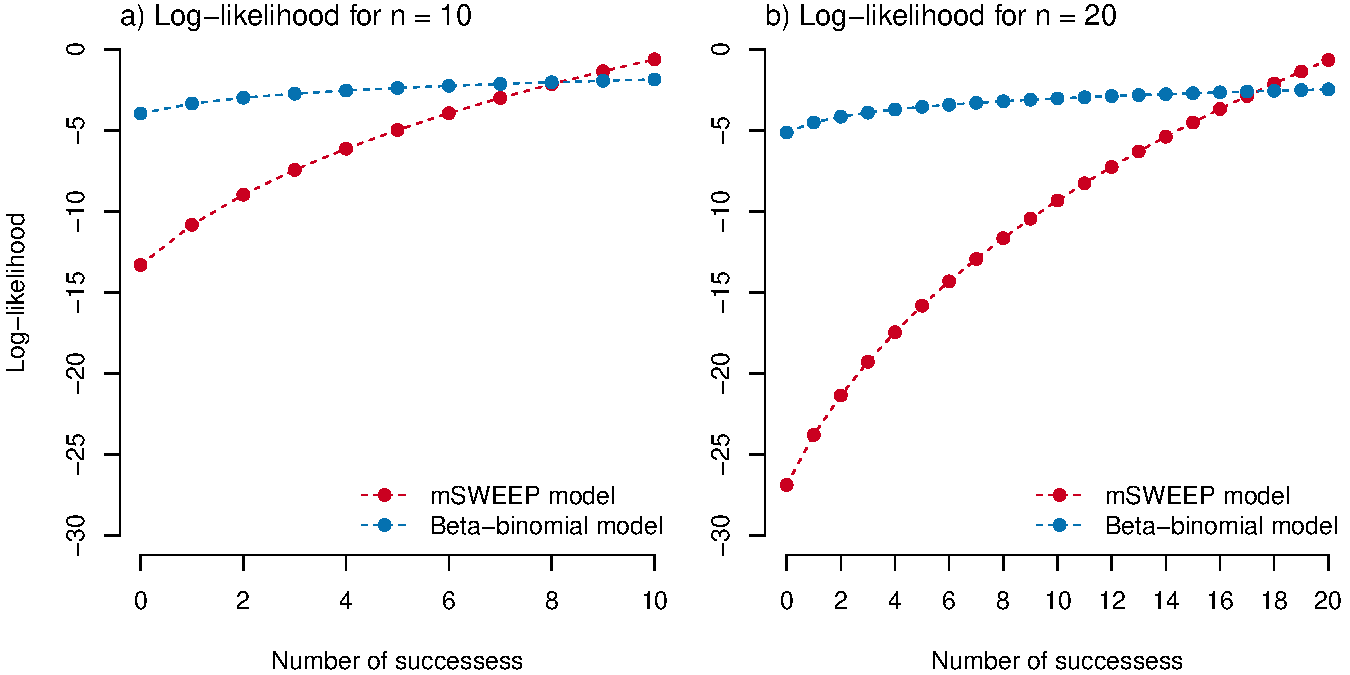
\includegraphics[width=\textwidth,keepaspectratio]{img/mSWEEP_likelihood.pdf}
    \caption{Comparison of the mSWEEP likelihood and a plain beta-binomial likelihood (both without zero inflation). The figure displays the difference between the modified beta-binomial likelihood that mSWEEP uses (red dots and lines) and a plain beta-binomial likelihood (blue dots and lines) with the same parameters. Panel \textbf{a)} displays the difference for a cluster with 10 reference sequences, and panel \textbf{b)} for a cluster with 20 reference sequences.}
\end{figure}

A comparison of the likelihood presented in Equation
\eqref{likelihood:beta-binomial-scaled} with the plain beta-binomial
likelihood in Equation \eqref{likelihood:beta-binomial-pmf} is presented
in Figure \ref{fig:msweep-vs-beta-binomial}. Figure
\ref{fig:msweep-vs-beta-binomial} shows that the mSWEEP format gives
more weight to values of $k$ that are close to $n$ while making the
differences between the different $k$ steeper than the plain
beta-binomial. In practice, the modified format implies that the
clusters should be defined in a way that most reads will pseudoalign
to the cluster if the read originated from the cluster but some
mismatches are still tolerated.

With the probability mass function of the distribution
$p^{\star}\left(k \middle| n, \alpha, \beta\right)$, the full
definition for the third part of the likelihood in Equation \eqref{likelihood:without-normalization} is
\begin{equation}
  \label{likelihood:normalized}
  p\left(r_{n, k} \middle| I_{n} = k\right) = 0.99\frac{p^{\star}\left(r_{n, k} \middle| M_{k}, \alpha, \beta\right)}{Z\left(r_{n, k}\right)}\text{ if } r_{n, k} \geq 1\text{ and } M_{k} > 1,
\end{equation}
where $Z\left(r_{n, k}\right)$ is a normalizing constant. The scaling
in Equation \eqref{likelihood:beta-binomial-scaled} fulfills the
requirement that the likelihood of each cluster must be on the same
scale despite different size. The next section will derive a closed
form for the normalizing constant $Z\left(r_{n, k}\right)$.

\subsection{Normalizing the likelihood}

While the function $p^{\star}\left(k \middle| n, \alpha, \beta\right)$
in Equation \eqref{likelihood:beta-binomial-scaled} closely resembles
the probability mass function of a beta-binomial distribution
(Equation \eqref{likelihood:beta-binomial-pmf}), the function
$p^{\star}\left(k \middle| n, \alpha, \beta\right)$ by itself does not
sum to $1$ over its support $k \in \left\{ 1, \dots, K \right\}$,
which means that the function is not a proper probability mass
function. To remedy this, the normalizing constant $Z\left(r_{n,
  k}\right)$ is needed.

In principle any distribution on a finite support can be normalized
but in many cases the normalizing constant does not have a closed
form. Fortunately, it turns out that \textemdash{ } thanks to the
properties of the beta function (see Equation
\eqref{likelihood:beta-function} for the definition) \textemdash{ }
$Z\left(r_{n, k}\right)$ does have a closed form. Deriving this closed
form requires using the following identity for the beta function
\begin{theorem}
  \label{lemma:beta-function-identity}
  \[
  B\left(a + 1, b\right) = \frac{a}{a + b}B\left(a, b\right).
  \]
\end{theorem}

\begin{proof}
  Follows from $B\left(a, b\right) = \frac{\Gamma\left(a\right)\Gamma\left(b\right)}{\Gamma\left(a + b\right)}$ \citep{artin_einfuhrung} and $\Gamma\left(z + 1\right) = z\Gamma\left(z\right), \text{ for all } z > 0$ \citep{davis_leonhard}, where $\Gamma\left(z\right)$ is the gamma function $\Gamma\left(z\right) = \int_{0}^{\infty}x^{z - 1}e^{-x}dx, z > 0$. Using these two identities, $B\left(a + 1, b\right)$ can be written as
  \begin{align*}
    B\left(a + 1, b\right) &= \frac{\Gamma\left(a + 1\right)\Gamma\left(b\right)}{\Gamma\left(a + b + 1\right)} \\
    &= \frac{a\Gamma\left(a\right)\Gamma\left(b\right)}{\left(a + b\right)\Gamma\left(a + b\right)} \\
    &= \frac{a}{a + b}B\left(a, b\right).
  \end{align*}
\end{proof}

Applying Theorem \eqref{lemma:beta-function-identity} leads to the closed form of the normalizing constant $Z\left(r_{n, k}\right)$.
\begin{theorem}
  \label{theorem:likelihood-can-be-normalized}
  Let
  \[
  f\left(k, n\right) = \binom{n}{k}\frac{B\left(\alpha + k, n - k + \beta\right)}{B\left(\alpha + n, \: \beta\right)}, 0 \leq k \leq n, \: \alpha > 0, \: \beta > 0,
  \]
  \text{and}
  \[
  Z\left(n\right) = \prod_{j = 1}^{n}\frac{\alpha + n + k - j}{\alpha + \beta + 2n - j},
  \]
  \text{then}
  \[
  \sum_{k = 0}^{n}\frac{f\left(k, n\right)}{Z\left(n\right)} = 1.
  \]
\end{theorem}

\begin{proof}
  Consider a beta-binomial distribution with the parameters $\left(n, \alpha + n, \beta\right), n \in \mathbb{N}_{+}, \alpha > 0, \beta > 0$. This distribution has the probability mass function $g : 0, \dots, n \rightarrow \left(0, 1\right)$, where
  \[
  g\left(k \: \middle| \: n, \alpha + n, \beta\right) = \binom{n}{k} \frac{B\left(\alpha + n + k , n - k + \beta\right)}{B\left(\alpha + n, \beta\right)},\: 0 \leq k \leq n.
  \]
  Using the identity $B\left(a + 1, b\right) = B\left(a, b\right)\frac{a}{a + b}, a > 0, b > 0$ (Lemma \eqref{lemma:beta-function-identity}) results in an alternative form for $g$
\begin{align*}
  g\left(k\right) &= \binom{n}{k} \frac{B\left(\alpha + n + k , n - k + \beta\right)}{B\left(\alpha + n, \beta\right)} \\
  &= \binom{n}{k} \frac{B\left(\alpha + n + k - 1 , n - k + \beta\right)}{B\left(\alpha + n, \beta\right)} \frac{\alpha + n + k - 1}{\alpha + n + k - 1 + n - k + \beta} \\
  &= \binom{n}{k} \frac{B\left(\alpha + n + k - 1 , n - k + \beta\right)}{B\left(\alpha + n, \beta\right)} \frac{\alpha + n + k - 1}{\alpha + \beta + 2n - 1} \\
  &= \binom{n}{k} \frac{B\left(\alpha + n + k - 2 , n - k + \beta\right)}{B\left(\alpha + n, \beta\right)} \frac{\alpha + n + k - 1}{\alpha + \beta + 2n - 1} \frac{\alpha + n + k - 2}{\alpha + \beta + 2n - 2} \\
  &= \binom{n}{k} \frac{B\left(\alpha + n + k - 2 , n - k + \beta\right)}{B\left(\alpha + n, \beta\right)} \prod_{j = 1}^{2} \frac{\alpha + n + k - j}{\alpha + \beta + 2n - j}.
\intertext{Above, Lemma \eqref{lemma:beta-function-identity} was applied twice. Repeadetly applying Lemma \eqref{lemma:beta-function-identity} $n$ times yields the alternative form}
  g\left(k\right) &= \binom{n}{k} \frac{B\left(\alpha + n + k - n , n - k + \beta\right)}{B\left(\alpha + n, \beta\right)} \prod_{j = 1}^{n} \frac{\alpha + n + k - j}{\alpha + \beta + 2n - j} \\
  &= \binom{n}{k} \frac{B\left(\alpha + k , n - k + \beta\right)}{B\left(\alpha + n, \beta\right)} \prod_{j = 1}^{n} \frac{\alpha + n + k - j}{\alpha + \beta + 2n - j} \\
  &= f\left(k, n\right) \prod_{j = 1}^{n} \frac{\alpha + n + k - j}{\alpha + \beta + 2n - j}.
\end{align*}
Since $g\left(k\right)$ is a probability mass function, this implies that
\[
f\left(k, n\right)\left(\prod_{j = 1}^{n}\frac{\alpha + n + k - j}{\alpha + \beta + 2n - j}\right)^{-1}
\]
is also a probability mass function. Thus, setting
\[
Z\left(n\right) = \prod_{j = 1}^{n}\frac{\alpha + n + k - j}{\alpha + \beta + 2n - j}
\]
is sufficient to normalize $f\left(k, n)$ and prove Theorem \eqref{theorem:likelihood-can-be-normalized}.
\end{proof}

\subsection{Likelihood hyperparameters}

Instead of the traditional parametrization for the beta binomial
distribution through $\alpha >0, \beta > 0$, in the mSWEEP paper the
distribution is reparametrized to slightly change the interpretation
of the parameters. The reparametrised forms for $\alpha$ and $\beta$ are
\begin{equation}
  \label{likelihood:reparametrization}
  \pi = \frac{\alpha}{\alpha + \beta}, \phi = \frac{1}{\alpha + \beta},
\end{equation}
where the first parameter $\pi$ has the range $\pi \in \left(0,
1\right)$ unless constraints are placed on $\alpha$ and $\beta$ and
represents the mean success rate in repeated draws from the beta
binomial distribution. The second parameter $\phi > 0$ measures
the variation in the success rate for each draw
\citep{griffiths1973maximum}. In the formulation for the likelihood in
Equation \eqref{likelihood:normalized}, each cluster $k$ has its own
parameters $\pi_{k}, \phi_{k}$.

Although methods such as Bayesian optimization (TODO citation) could
be employed to find optimal values for the parameters $\pi_{k},
\phi_{k}$ in Equation \eqref{likelihood:reparametrization}, we set their
values based on a reasonable compromise that performed well in the
mSWEEP paper. The values of $\pi_{k}, \phi_{k}$ are set to
\begin{equation}
  \begin{aligned}
    \pi_k &= 0.65, \text{ for all } k = 1, \dots, K, \\
    \phi_{k} &= 1 - \pi_{k} + 0.01M_{k}^{-1}.
  \end{aligned}
\end{equation}

\subsection{Fitting the model using variational inference}

With the likelihood defined in Equations
\eqref{likelihood:without-normalization} and
\eqref{likelihood:normalized}, all that remains is to come up with a
suitable method to infer the relative abundances
$\boldsymbol\theta$. Since the model is principally the same as the
one used in BIB (Equation \eqref{model:grouped-joint-distribution}),
just with a different formula for the likelihood term $p\left(r_{n, k}
= k \middle| I_{n} = k\right)$, the variational inference algorithm
from BIB can be adjusted by simply changing the likelihood term to
that of Equation \eqref{likelihood:without-normalization} and the rest of
the algorithm remains the same.

Variational inference by itself is an extremely broad topic that lies
somewhat outside the scope of this dissertation. Thus, I will only
cover the parts that are directly relevant to the contributions from
the thesis \textemdash{ } namely, how the probability matrix that mSWEEP
generates and mGEMS leverages is obtained. For a more thorough
coverage of variational inference in this context, the BitSeqVB paper
\citep{hensman2015fast} provides an explanation for the case where the
algorithm is derived for the same model, only with a different
likelihood function.

In brief, variational inference for the mSWEEP model consists of
finding a distribution $q\left(\boldsymbol\theta, I\right)$ that
minimizes the Kullback-Leibler divergence to the true posterior
$p\left(\boldsymbol\theta, I \middle| R\right) \approx
q\left(\boldsymbol\theta, I\right)$. For simplicity, assume that the
approximation $q\left(\boldsymbol\theta, I\right)$ factorizes into
$q\left(\boldsymbol\theta, I\right) =
q\left(\boldsymbol\theta\right)q\left(I\right)$. Because each $I_{n}$
has a categorical distribution $Cat\left(\boldsymbol\theta\right)$ and
they are furthermore assumed independent of each other, $I_{n} \indept
I_{m}, n \neq m$, the second term $q\left(I\right)$ simplifies to
\begin{equation}
  \label{likelihood:vi-factorization}
  q\left(I\right) = \prod_{n = 1}^N\prod_{k = 1}^K \gamma_{n, k}^{I_{n, k}}.
\end{equation}

In practice, the best approximation $q\left(\boldsymbol\theta,
I\right)$ is found when optimal values for the parameters $\gamma_{n,
  k}$ in Equation \eqref{likelihood:vi-factorization} are found (TODO
cite). The Riemannian conjugate gradient (RCG) method is used to find the
optimal values for $\gamma_{n, k}$ (TODO cite). A generic and parallel
\& distributable implementation for arbitrary likelihood with this
mixture model structure is available from
\url{https://github.com/tmaklin/rcgpar}.

\subsection{Alternative fit using MCMC sampling}
Alternatively, the model could be fitted using Markov chain Monte
Carlo (MCMC) sampling methods (TODO citations or explain). Instead of
the variational inference approach of finding an approximating
distribution $q\left(\boldsymbol\theta, I\right)$, MCMC sampling
attempts to produce a set of samples from the true posterior
$p\left(\boldsymbol\theta, I\middle| R\right)$. Averaging over the
values produced via MCMC sampling $\hat{\boldsymbol\theta}$
(asymptotically) produces the true parameters $\boldsymbol\theta$ as
the number of samples increases.

Even though producing the true values is tempting, MCMC has several
problems when applied in practice (TODO citations). First, the true
values are only found asymptotically, meaning that it is difficult to
determine when the MCMC sampler has converged to the true
posterior. Secondly, due to the first point, the number of samples
that need to be drawn may be excessively high, resulting in long run
times when compared to the significantly faster variational inference
(TODO cite, variational inference for statisticians paper?).

Compared to variational inference, MCMC does have the advantage that,
provided sufficient runtime, the samples will be from the true
posterior. In practice, this leads to better estimates of the
covariance between the sampled parameters when the model is of the
form in Equation \eqref{model:joint-distribution} (cite BitSeqVB
paper). However, replacing the variational inference algorithm in the
mSWEEP model with the Gibbs sampler from the original BitSeq
\citep{glaus2012identifying} does not seem to produce any significant
differences between the parameter estimates (Figure TODO gibbs vs vi).

\textbf{TODO: - Add figure of Gibbs sampler vs variational inference experiments.}

\section{From profiling to binning}
\label{section:binning}

This sections covers using the model from mSWEEP to derive an
algorithm for assigning the sequencing reads $r_{n, k}$ to the
reference lineages $k$, also known as binning. Binning differs from
relative abundance estimation in that the goal is to produce some
assignment of the reads to reference units. Typically the reference
units and the created bins correspond to some species or even
genuses. In this thesis, the bins will be created on the level of the
reference lineages/clusters that mSWEEP reports the relative
abundances for. Compared to estimating only the abundances, the
addition of binning provides much extra detail about the contents of a
sample, since the creation of lineage-level sequencing read bins
allows performing many downstream analyses that require sequencing
reads or even assemblies. The binning algorithm presented in this
section is called the mGEMS binning algorithm, which in itself is a
part of the mGEMS pipeline for binning sequencing reads.

The work in this section is based on the results from the second paper
included in the dissertation \citep{maklin_bacterial_2021}. Compared
to the previous section presenting the mSWEEP probabilistic model, the
binning algorithm is somewhat more straightforward.

\subsection{The mGEMS binning algorithm}

A crucial feature for the binning algorithm to handle lineage-level
differences between bacteria is that the algorithm must allow for
assignment of a single read to multiple bins at the same time. Because
of the relatively small differences between different lineages of a
bacterial species, the read could easily have been generated from
several of them. This differs from most work on binning, where the
reads are typically only allowed an assignment in a single bin at a
time because the variation between the organisms belonging to
different bins is assumed large enough that multi-bin assignment is
not necessary (TODO citations). For within-species-level binning, this
assumption obviously does not hold because of the shared genomic
contents when the species are defined in a manner that reflects their
phylogenetic characteristics. This means that the mGEMS binning
algorithm must be explicitly defined in a way that allows for
assignment to multiple bins.

The mGEMS binning algorithm consists of a rule for assigning the reads
to the bins. This rule is derived by leveraging the read-level
assignment probabilities $\gamma_{n, k} \in \left(0, 1\right)$, $n =
1, \dots, N$, $k = 1, \dots, K$, $\sum_{k = 1}^{K}\gamma_{n, k} = 1$
produced by the variational approximation used in fitting the mSWEEP
model (Equation \eqref{likelihood:vi-factorization}). To derive the
assignment rule, some further assumptions regarding the reads and the
reference sequences are required. Firstly, the sequencing reads are
assumed to contain only one member of the same lineage \textemdash{ }
similarly to the typical metagenomic binners assuming only variation
at the level they operate on. Secondly, should the true reference
sequence that generated the reads be missing from the reference, the
set of reference sequences in the lineage that generated the reads is
assumed to adequately cover the variation in the missing sequence. The
second assumption is necessary since reads that do not pseudoalign to
any reference sequence in the collection are discarded by mSWEEP.

To fulfill our requirement that a read can be assigned to several bins
at the same time, the bins $G_{k}$ for each cluster $k$ are defined as
a subset of sequencing reads $r_{n}$ such that
\begin{equation}
  \label{binning:bins-definition}
  G_{k} = \left\{r_{n} : \gamma_{n, k} \geq q_{k}\right\}
\end{equation}
holds for some threshold $q_{k} \in \left[0, 1\right]$. Note that the
threshold may be different for each cluster $k$. Because of the way
the bins $G_{k}$ are defined in Equation
\eqref{binning:bins-definition}, this definition obviously allows for
a read to belong to several bins (for a trivial example, consider
the case where $q_{k} = 0$ for all $k$).

\subsection{Assignment rule for multi-cluster membership}

Next, the thresholds $q_{k}$ should be assigned some sensible value
that maximizes the probability $A_{n, k}$ of assigning the read
$r_{n}$ to the bin $G_{k}$ if the cluster $k$ (could have) generated
the read $r_{n}$. Ideally, the probabilities $A_{n, k}$ could be
defined through other probabilities $B_{n, k}$ with the meaning: the
cluster $k$ contains a sequence that contains the true (error-free)
nucleotide sequence of the read $r_{n}$. However, the probabilities
$B_{n, k}$ are quite difficult to estimate directly since 1) the reads
cannot be error-corrected with full accuracy, and 2) the reference
collection is nearly always incomplete. These two problems can be
remedied by assuming that the sample is composed mostly of closely
related organisms, which allows deriving the following relationship
between $A_{n, k}$ and $B_{n, k}$
\begin{equation}
  \label{binning:a-is-approximately-b}
  P\left[A_{n, k} = 1\right] \approx \theta_{k}P\left[J_{n, k} = 1\right],
\end{equation}
where $\theta_k$ is the relative abundance of the cluster $k$ in the
sample that generated the reads $r_{n}$. Equation
\eqref{binning:a-is-approximately-b} implies that when $P\left[A_{n, k}
  = 1\right] \geq \theta_{k}$, then $P\left[B_{n, k} = 1\right]$ must
be ``large'' for the approximation to hold. A more detailed derivation
for this statement about the magnitude of $B_{n, k}$ and Equation
\eqref{binning:a-is-approximately-b} is provided in the methods section
of the mGEMS article \citep{maklin_bacterial_2021}, supplied in the
appendix for this thesis and omitted from here.

The implied statement about the magnitude of $B_{n, k}$ when
$P\left[A_{n, k} = 1\right] \geq \theta_{k}$ means that there is a
high chance that $B_{n, k} \rightarrow 1$ when the former
holds. Because of this relationship, an assignment rule can be derived
by using the estimates $\gamma_{n, k}$ (Equation
\eqref{likelihood:vi-factorization}) for the probability $P\left[A_{n,
    k} = 1\right]$
\begin{equation}
  \label{binning:theoretical-assignment-rule}
  \text{if } \gamma_{n, k} \geq \theta_{k}, \text{ assign the read } r_{n} \text{ to } G_{k}.
\end{equation}
Equation \eqref{binning:theoretical-assignment-rule} provides an
inequality whose validity can be checked to assess the probability of
the event $B_{n, k} = 1$ which could not be estimated directly.

\subsection{Practical considerations}

While the assignment rule in Equation
\eqref{binning:theoretical-assignment-rule} provides a theoretically
sound tool to assign reads $r_{n}$ to the bins $G_{k}$, applying it in
practice requires a slight adjustment due to computational
accuracy. Namely, when estimating the relative abundances $\theta_{k}$
of $N$ reads, any estimate that falls below $\frac{1}{N}$ means that
zero reads originated from the cluster $k$. Because of this, values
$\theta_{k} < \frac{1}{N}$ are in some sense meaningless, and all
represent the same case of 0 reads from the clusters where the
inequality is true. Due to the constraint that $\theta_{k}$ must sum
up to $1$ over $k$, these essentially-zero values do, however,
contribute a small amount of noise to the other estimates that exceed
$\frac{1}{N}$. Since there are $K$ clusters, the fraction of noise $d$
is (in the worst-case scenario) at most
\begin{equation}
  \label{binning:assignment-rule-noise}
  d = (K - 1)\frac{1}{N}.
\end{equation}

The noise-level in the worst-case scenario of Equation
\eqref{binning:assignment-rule-noise} means that when evaluating the
validity of the inequality in Equation
\eqref{binning:theoretical-assignment-rule}, the thresholds $\theta_k$
should be adjusted with $1 - d$. This adjustment in turn means that
only the fraction of relative abundance that is assigned to nonzero
estimates in the wost-case scenario is considered. Adjusting Equation
\eqref{binning:theoretical-assignment-rule} with $d$ produces the final
assignment rule that is used in mGEMS
\begin{equation}
  \label{binning:assignment-rule}
  \text{if } \gamma_{n, k} \geq (1 - d)\theta_{k}, \text{ assign the read } r_{n} \text{ to } G_{k}.
\end{equation}
Because the variational approximation used to fit the mSWEEP model
already provides both the estimates $\gamma_{n, k}$ and the relative
abundances $\theta_{k}$, the assignment rule in Equation
\eqref{binning:assignment-rule} is in practice extremely inexpensive to
evaluate after the model has been fitted.

\subsection{General applicability of the assignment rule}

Since the relative abundances $\theta_k$ are derived from the values
$\gamma_{n, k}$ by averaging over $n = 1, \dots, N$, the assignment
rule in Equation \eqref{binning:assignment-rule} can be seen as a way to
cluster the rows (or columns) of a generic probability matrix, whose
rows (or columns) sum up to $1$. This rule in particular allows
assigning each row (or column) to several clusters at the same
time. However, more general applicability of the rule to probability
matrices is not explored further in this thesis beyond this
acknowledgement that the rule could be applied to more general
scenarios where a probability matrix needs to be clustered.

The next chapter will cover the application of mSWEEP and mGEMS to
different kinds of sequencing data and explore how the methods enable
new directions in analysis of sequencing data. The chapter also
includes a coverage of the benchmarks and experiments presented in the
first and second papers (TODO cite).

\chapter{High-resolution metagenomics}

High-resolution metagenomics (in the context of this thesis) refers to
applying some method capable of recovering variation at the
within-species level to some sort of metagenomics data as defined in
Section \ref{three-approaches-to-metagenomics}. In this chapter, the
methods of interest are mSWEEP and mGEMS. The chapter will deal with
the benchmarking and experimental results from the first two papers,
which focus on analysing plate sweep metagenomics data. At the end of
the chapter some technicalities arising from the model formulation
presented in Chapter 2 will also be covered. These mostly cover
questions about reliability of the results when applied to realistic
use-cases.

\section{Plate sweep and WGS metagenomics}

The primary methods for obtaining metagenomics sequencing data
considered are plate sweep metagenomics and whole-genome shotgun (WGS)
metagenomics (see Section \ref{three-approaches-to-metagenomics} for
more details). Of these two, plate sweep metagenomics has the
advantage of being able to focus sequencing efforts to species that
are known to grow on specific culture media, while WGS metagenomics
provides data of \textit{all} organisms on some sample (including for
example host DNA, fungi, commensal species, and so on). When the goal
is to investigate strain-level variation, both approaches have their
uses in either producing more data from the species of interest or
providing a less biased view of the sample contents at the expense of
sequencing depth. The first two papers included in the thesis were
written with only plate sweep metagenomics in mind but the third paper
demonstrated that mSWEEP and mGEMS are applicable in the WGS
metagenomics context. Thus, this chapter will not discriminate between
the two.

\subsection{Benefits of metagenomics over culturing}

When comparing metagenomics approaches to culturing isolates, the
major difference between the approaches is that metagenomics will
provide a better overview of the microbiome in the sample. Although
isolate data has mostly been used in the past in epidemiological
studies, some demonstrating the benefits of applying a metagenomics
approach have emerged. In particular, a recent study utilizing mSWEEP
might not allow identifying the presence of non-dominant variants of
the same species \citep{tonkin-hill_pneumococcal_2022}. Similar
approaches using other tools have also hinted at the capability of
several strains to become pathogenic should the opportunity present
itself (TODO citations? or remove). These studies have demonstrated
that it may be necessary to incorporate some level of metagenomics in
epidemiological studies in order to better identify the causative
agents (TODO citations) of disease.

Microbiome studies in general have become increasingly popular with
the advent and adoption of 16S sequencing (TODO citation). Although
the results of some studies remain somewhat controversial (TODO
citation), the widespread application of 16S metagenomics has revealed
extensive variation in the microbiome. Currently it is a somewhat of
an open question whether this naturally occurring variation extends to
the strain-level. Nevertheless, some studies both old and new have
demonstrated that this might be the case (TODO citations).

mSWEEP and mGEMS enable answering these questions regarding
strain-level variation by providing methods that can be targeted to
capture the variation present in samples containing members of some
bacterial species. Since many bacteria of clinical importance have
been studied for several decades (TODO citations) with significant
sequencing efforts aimed at them to obtain high-quality genome
assemblies (TODO citations), the reference-based approach employed by
mSWEEP and mGEMS is ideal for disentangling variation in the same
clinical setting. When combined with tools that take different
approaches to analysing metagenomic data, the combination has the
potential for providing unprecedented level of detail in future
epidemiological analyses and routine surveillance.

While the previous chapter covered the theoretical foundations of
mSWEEP and mGEMS, the remainder of this chapter will focus on the
practical considerations regarding these two methods. Namely, we
briefly overview the performance of the methods in various settings,
and cover some questions related to the reliability of the approach as
well as the sensitivity to the reference sequence collection. The last
part of the chapter will provide some extra coverage of the results
from the included papers, with the aim of exploring what kind of
information metagenomics-derived results provide.

\subsection{The mSWEEP/mGEMS pipeline}
\textbf{TODO: - Flowchart describing the analysis pipeline.}

Combining the results from Sections \ref{section:model} and
\ref{section:binning} produces the complete mSWEEP/mGEMS workflow for
analysing sequencing data from mixed sources. This workflow is
originally presented in the second paper
\citep{maklin_bacterial_2021}, where it is referred to as the mGEMS
pipeline.

\subsubsection{Constructing the reference database}

The pipeline begins with constructing a set of reference sequences
that represent the variation in the target species of interest. In an
ideal scenario, the reference should consist of high-quality
assemblies from each lineage that is expected to be found in the
sequencing reads. Since this is a rather unrealistic assumption,
typical cases make use of published datasets and possibly combine them
with isolate sequencing data from their own studies. Either previously
published assemblies, or even curated genomes from databases such as
RefSeq (TODO citation?), may be used. The reference may also include
newly assembled sequences or otherwise be tailored to the problem at
hand. In both cases, a cautious approach is recommended, as the
quality of the reference sequence collection is the most important
factor in obtaining trustworthy results from the pipeline.

After the appropriate reference sequences have been collected, they
should be clustered in some meaningful way to obtain the lineage
grouping. For some species, multilocus sequence typing is sufficient,
but for others with more variable genome contents, algorithms that
attempt to identify clonal complex analogues (central multilocus
sequence type and its 1 or 2 locus variants) may be useful. One such
algorithm is PopPUNK \citep{lees2019fast}, which is demonstrated to
perform well in the third paper of this thesis. PopPUNK clusters the
reference sequences based on accessory and core genome distances with
an option to perform the clustering only based on the core-genome. The
resulting clustering from PoPPUNK is similar to clonal complexe. Using
a computational like PopPUNK instead of a curated database approach
like the sequence types and clonal complexes has the advantage of
providing means to assign sequences that have not yet been included in
the curated databases, or work with species for which such databases
do not exist.

After clustering the reference sequences, the next step is to build an
index for pseudoalignment, and pseudoalign the reads from the samples
against the index. In the mGEMS pipeline, we use Themisto
\citep{maklin_bacterial_2021} to perform both the index construction
and the pseudoalignment. The pseudoalignment step produces binary
pseudoalignment vectors for each read against every reference
sequence, which are used as the input to mSWEEP.

\subsubsection{Estimating relative abundances and binning the reads}

The next step in the pipeline is to use mSWEEP to estimate the
relative abundances of the reference groups based on the
pseudoalignments. This is performed directly on the output from
Themisto, with no intermediate steps required. After the relative
abundances have been estimated, the results are fed to mGEMS which
produces the read bins and optionally also extracts the reads
corresponding to each bin from the original set.

\subsubsection{Assembling the read bins}

In the second paper of this thesis, the mGEMS pipeline also contains
an optional step to assemble the reads placed in each bin. The
suggested assembler is shovill (TODO citation), which is an assembly
pipeline built around the spades assembler (TODO citation) but
incorporates some pre- and post-processing steps (TODO
citations). Naturally, other assemblers may also be used, or the
assembly step skipped entirely and the analysis instead focused on the
reads. In the second paper, the analyses mostly focused on using the
assemblies, as including an assembly step is equivalent to adding a
post-processing step that aids in filtering out reads that may
mistakenly have been assigned to the wrong bin.

Since mGEMS allows for assigning a sequencing read to several
bins/lineages at once, the produced bins sometimes have very high
coverages for the the genomes that the organisms corresponding to the
bins share. This is especially true when the sample truly contains
several closely related organisms. Consequently, we investigated in
the second paper the effect of replacing the isolate-data optimised
shovill with metagenomic assemblers (TODO citations), which presumably
implement better handling of variable coverage in the produced
genomes. Although we observed some differences in the resulting
assemblies (TODO reproduce figure here?), there was no statistically
significant evidence in favour of using either approach. Regardless of
the assembler choice, using the assemblies from the mGEMS pipeline in
downstream analyses performed similarly to using those created from
corresponding isolate sequencing data.

\subsubsection{Quality control}

The mGEMS pipeline as described above is the method that has been
applied in the third paper with the additional inclusion of a quality
control (QC) step attempting to identify whether the reference
sequences suitably cover the variation in the sequencing reads. This
QC step, called demix\_check
(\url{https://github.com/harry-thorpe/demix_check/}) (TODO move to
footnote), performs several checks on the results from mSWEEP and
mGEM, to determine whether the created read bins correspond to some
reference cluster. Although the demix\_check step was not used in the
two methods papers presenting mSWEEP and mGEMS, its inclusion
addresses an important question regarding the applicability of the
results from mSWEEP/mGEMS (TODO cite review from mSWEEP
paper?). Therefore, including demix\_check \textemdash{ } or other
similar approach \textemdash{ } as part of the mGEMS pipeline between
the mGEMS and the assembly steps is recommended for a rigorous
approach. This and other questions related to quality control and
reliability of the results are explored further down in this chapter.

\textbf{TODO:- figure from showing the threshold construction process.}

\subsection{Other approaches for metagenomic analyses}
\label{other-metagenomics-approaches}
While this thesis deals with the development and usage of mSWEEP and
mGEMS, one has to acknowledge that the use of metagenomic sequencing
data is by no means an understudied field. In fact, dozens of methods
exist that aim to perform similar tasks ranging from genome assembly
from metagenomic sequencing data (metagenome assemblers) (TODO
citations) to taxonomic binning (metagenomic binners) (TODO citations)
and profiling (TODO citations), and strain tracking (StrainGE and
Strainphlan) (TODO citations). Compared to mSWEEP and mGEMS, these
methods typically assume that the samples only contain a single strain
from each species \textemdash{ } with the exception of StrainGE, which
explicitly addresses the presence of several strains \textemdash{ },
which enables them to solve the task when the assumption holds. While
it may at first seem suspicious that a thorough comparison between
these methods and mSWEEP/mGEMS has not been included in the published
papers, the assumptions about the strain complexity lie at the heart
of the questions addressed by mSWEEP and mGEMS. Since the preceding
metagenomics tools have typically not been developed with the
strain-complexity in mind in mind, a performance comparison between
them is not meaningful nor fair.

\section{Benchmarking mSWEEP and mGEMS}
% WIP continue from here

This section will briefly cover the results related to benchmarking
the performance of mSWEEP and mGEMS in the first and the second
papers. A majority of the benchmarks were performed on synthetic
mixtures of sequencing reads from isolate cultures but the mGEMS paper
also provides a (significantly smaller in scale) benchmark that used
\textit{in vitro} mixtures of DNA from isolate cultures. Figures from
the papers have not been reproduced here, and the results are
presented in a summarizing format merely to convince the reader of the
kinds of applications that mSWEEP and mGEMS perform well in.

\subsection{mSWEEP}
The first paper in the thesis presented a comparison of mSWEEP with
the Bayesian Identification of Bacteria (BIB) and the
pseudoalignment-based metakallisto methods. Although a myriad of
taxonomic profilers have been developed (these will be covered in more
detail in Section \ref{other-metagenomics-approaches}), the vast
majority of them do not attempt within-species profiling or have been
developed for cases with only one strain present from each
species. Because of these limitations, the mSWEEP paper only makes the
comparisons with BIB and metakallisto, which have been developed for
settings with several strains present.

While the approach in BIB is similar to mSWEEP in that the reference
sequences are grouped together and estimation is performed on the
level of these groups, metakallisto attempts the much more ambitious
task of estimating the relative abundances for the individual
sequences. Because of this, a direct comparison between the three is
not possible. We addressed this issue by modifying the output from
metakallisto by including a step that sums over the abundance
estimates within the same group. Even though this step was not
included in the original metakallisto paper, its addition helps to
compare the estimates from mSWEEP, BIB, and metakallisto.

The main result of the first paper is that mSWEEP vastly outperforms
both BIB and metakallisto for most species. For species with a
strictly defined clonal structure \textemdash{ } such as
\textit{S. aureus} \textemdash{ }, BIB and metakallisto are able to derive
comparable performance, but for other species that exhibit more varied
clonal structures incorporating the probabilistic model from mSWEEP
proves to be a necessary step in obtaining accurate
information. Although these performance benchmarks were only performed
on data containing a single strain in each sample, we demonstrate in
the paper through stochastic dominance that the methods which do not
succeed with single-strain estimates are unlikely to provide accurate
results from multi-strain samples.

Another benchmark presented in the first paper concerns evaluating
performance in the presence of several strains from the same
species. In this benchmark, sequence data from three strains were
mixed together in single sample at known proportions, and mSWEEP was
applied to estimate the proportions when the real reference sequences
were absent from the reference data but close representatives from the
same lineage were available. In this benchmark, mSWEEP demonstrates
very accurate performance measured on both true positives and true
negatives. Although \textit{K. pneumoniae} in particular proved
challenging, possibly due to the wide variety exhibited in the
reference set, the results were nevertheless within acceptable error

In addition to the synthetic experiments presented in the first paper,
the second paper presents an \textit{in vitro} benchmark concerning
abundance estimation. In this benchmark DNA from three different
strains of either \textit{E. coli} or \textit{E. faecalis} was mixed
together using Qbit, producing samples where the initial composition
of the sample is known at the DNA level. This benchmark shows similar
results as the synthetic benchmarks for \textit{E. faecalis}, where
the three strains originated from three different sequence types, but
also shows promise in differentiating between strains of the same
clade within a single sequence type of \textit{E. coli}. This task is,
however, much, much more difficult since the split of the ST131
subclade C2 was based on incorporating information from the accessory
genome using PopPUNK. The accessory genome of \textit{E. coli} is not
as stable as the core genome, on which the ST131 and the ST131 A-C
designations are based, resulting in some difficulties in separating
the C2-4 and C2-6 sublineages. Nevertheless mSWEEP manages to identify
the presence of both clades quite well, and the downstream analysis
using mGEMS (covered in Section \ref{mgems-performance-benchmark}
still provides accurate results.

\subsection{mGEMS}
\label{mgems-performance-benchmark}

Our taxonomic binner mGEMS was benchmarked in the second paper using
both synthetic data (mixtures of reads from isolate cultures of
different strains) as well as the previously mentioned \textit{in
  vitro} benchmark. The chief metrics used were related to those that
are the main objects of interest in genomic epidemiological analyses:
SNPs and phylogenies estimated from the SNP data. We looked at the
performance of mGEMS on the level of within-ST variation using data
from \textit{E. coli} (TODO cite paper), at the between-ST and
within-species level using \textit{E. faecalis}, and an extreme case
with only dozens of SNPs separating the different reference clusters
using data from \textit{S. aureus}.

\subsubsection{Synthetic data benchmarks}

In the \textit{E. coli} benchmark we investigated how well
mGEMS-derived assemblies performed for maximum likelihood phylogeny
estimation (using RAxML-NG, Gamma+GTR4M model) when compared to using
isolate sequencing data. We used snippy to derive the core genome
alignment against the same reference genome for both mGEMS-derived
assemblies and the isolate assemblies. The results showed that mGEMS
tends to slightly overestimate the number of SNPs in these assemblies
(Figure 2 panel a in the paper (TODO cite)) but the phylogenetic
relationships (Figure 3) are recovered quite well. This benchmark was
performed at the level of variation within a sequence type
(\textit{E. coli} ST131).

The \textit{E. faecalis} benchmark was performed similarly to the
\textit{E. coli} one but with the intention of investigating
performance with between-ST variation. Additionally,
\textit{E. faecalis} is known to have a relatively high rate of
recombination within the species across ST lines (TODO citation),
which adds to the difficulty of the problem. Nevertheless, the mGEMS
derived-assemblies do recover the overall structure of the phylogeny
and place to sequences from the same ST to the same clade. While the
global structure is somewhat different from the isolate assembly
phylogeny, these kind of differences may easily be explained by
uncertainty arsing from recombination affecting the placement of the
STs globally. This phenomenon is also apparent in the bootstrap
support values for both the isolate and mGEMS-derived phylogenies.

The final synthetic benchmark in the second paper investigated
phylogeny recovery in \textit{S. aureus} ST22 sublineages that are
separated by a few dozen SNPs (TODO citation). Although the
performance in this benchmark was not quite as good as in the two
others, the mGEMS-derived results nevertheless do manage to replicate
some parts of the results relating to the transmission analysis
performed in the source study for this data. Namely, the samples that
were observed to be the likely source of the pathogenic strain in the
sequenced patients were placed at the root of the phylogeny when using
both mGEMS and isolate data. Regardless, there is some lack of detail
further down in the tree which is likely a result of the small degree
of separation between the sublineages.

\subsubsection{\textit{In vitro} benchmark}

The second paper also included an \textit{in vitro} benchmark data,
where known amounts of DNA from three different strains were mixed
together using Qbit, and both the mixed sample and the corresponding
isolate cultures were sequenced. This data was used to re-test the
performance of both mSWEEP (covered in the previous subsection) and
mGEMS. The mGEMS part of the test examined the recovery of SNPs from
either the isolate sequencing data or the mixed sequencing data. In
both the \textit{E. coli} and \textit{E. faecalis} test samples the
SNPs recovered from the mGEMS data reflect the ``true'' values from
the isolate data quite closely, although there is some difficulty in
separating the ST131-C2 sublineages 4 and 6. However, due to the
increasingly difficult task of defining sublineages within
sublineages, this difficulty is likely not relevant for practical
analyses.

Together, these benchmarks hopefully show that the mGEMS method can be
reliably used to disentangle metagenomic sequencing data and create
lineage-specific read bins. These bins in turn can be used in standard
epidemiological analyses in place of isolate sequencing data,
producing similar results. While mGEMS does not completely replace the
use of isolate sequencing data in epidemiology \textemdash{ } the
availability of high-quality reference sequences from isolate
sequencing remains a critical part of the pipeline \textemdash{ } the
method nevertheless shows promise in reducing the number of isolate
cultures that need to be created. Additionally, applying mGEMS to pure
metagenomics sequencing data can yield results that previously
available tools have not been able to produce as will be shown in more
in Chapter \ref{section:metagenomic-epidemiology} that covers the
experimental results from the third paper.

\section{Assessing reliability of the results}

A principal question when applying mSWEEP/mGEMS in practice is whether
the results from either are trustworthy or not. Since the former
method uses a Bayesian approach to estimating the relative abundances
of the reference lineages, none of the abundances will ever be exactly
zero. This naturally results in the question: ``When is a lineage
truly present in the sample?'' when applying mSWEEP in
practice. Furthermore, since the abundance estimates from mSWEEP are
the basis for the mGEMS pipeline, it is of importance to know when the
results for lineages with a high (in some sense) relative abundance
are truly correct and not just a result of, for example, missing
reference lineages. These two questions will be covered in the rest of
this section.

\subsection{Detection thresholds for lineages}
To answer the question regarding the minimum abundance required to
call an abundance estimate reliable or not, the mSWEEP paper provides
an approach termed \textit{detection thresholds}. These thresholds aim
to provide a minimum abundance that the estimates must exceed in order
to be reliable, and give accompanying p-value-analogues to assess the
degree of trust in the threshold itself. Although this approach is
computationally somewhat cumbersome to apply in practice, especially
when the size of the reference sequence set increases, the approach
should nevertheless provide means for more careful consideration of
the estimates without resorting to simpler measures such as filtering
by a constant abundance.

The detection threshold approach is based on bootstrapping sequencing
reads from existing samples with known genome assemblies in the
reference collection. The assembly is removed from the reference, and
the bootstrapped reads (which contain data from only the single,
removed assembly) are put through mSWEEP to obtain a bootstrapped
abundance estimate. This approach is then repeated for some number of
reference sequences, each removed in turn, to provide several
bootstrapped abundance estimates for each reference lineage. The
bootstrapped estimates are used to evaluate the magnitude of the
relative abundance estimates that are given for the \textit{absent}
lineages, and combined across all values generated when varying the
removed reference sequences. When repeated for all reference lineages,
this approach gives a set of values that represent the false estimates
when the true contents of the sample are different. The false estimates
for each lineage are ordered, and one of the higher values is picked
as a cutoff point that defines the detection threshold for this
lineage with an accompanying p-value-analogue that depends on the
number of estimates that are allowed to exceed the cutoff. This
somewhat complicated approach is described in more detail in the first
paper.

While the detection thresholds approach has some merit in its
theoretical foundations in using bootstrapping to estimate the
magnitude of the false estimates, the approach has some problems when
applied in practice. Namely, the need to remove a reference sequence
to bootstrap the abundance estimates necessitates reconstruction of the
pseudoalignment index for each sample that is generated from the
removed sequences. Since dynamic indexing (meaning that sequences can
be added/removed without rebuilding the whole index) remains an open
problem at the time of writing, the approach is quickly rendered
computationally infeasible when applied to reference sets that are
larger than those used in the mSWEEP paper. Unfortunately for the
detection threshold construction, for many applications it is tempting
to include as much reference data as possible to cover naturally
occurring strain-level variation. This has resulted in the approach
being not applied in practice and remaining a curiosity until dynamic
indexes hopefully become available.

\subsection{Pseudocoverage as a threshold}

One alternative to the detection thresholds can be found by figuring
out a way to define some sort of threshold on the abundance estimates
without utilizing bootstrapping-based approaches. In practice, this
translates to using the number of aligned reads and the abundance
estimates together to estimate the \textit{pseudocoverage} of the
reference lineage. Pseudocoverage $c^{\star}_{k}$ for reference
lineage $k$ is defined as the product of the abundance estimate
$\theta_{k}$ for lineage $k$ and the total number of bases $b$ in the
reads that pseudoaligned against any reference sequence divided by the
average genome length $l_{k}$ in lineage $k$
\begin{equation}
  \label{pseudocoverage}
  c_{k}^{\star} = \frac{\theta_{k}b}{l_{k}}.
\end{equation}
Although the definition in Equation \ref{pseudocoverage} is similar to
the basic definition of average coverage (number of bases in aligned
reads divided by genome length), these two definitions are not
necessarily the same.

To elucidate the difference between coverage and pseudocoverage,
consider a set of sequencing reads originating from two bacterial
strains, both with $100$ base pair long genomes, that differ by a
single base pair and are present in equal proportions in the sample
providing the sequencing reads. Assuming that we have 100 one base
pair long reads from each position in both genomes, the average
coverage of both strains would be $199$ since $9900\cdot2$ reads
will align to both genomes and only $100\cdot2$ reads will align to
just one. However, when considering the relative abundance estimates
for these two strains, their true values are $0.50$ and $0.50$ since
we know that both strains are present in equal proportions. This gives
both strains a pseudocoverage of $99.5$ \textemdash{ } a conservative
value compared to the traditional coverage definition.

Pseudocoverage can be used to define a threshold on the relative
abundance estimates by finding the value of $\theta_{k}$ that provides
for example a pseudocoverage of \textit{at least} $1$x. Since the
pseudocoverage is a conservative estimate of the true coverage (the
exact, typically more complex than in the thought experiment above,
relationship depending on the relatedness of the lineages $k$), this
minimum value can be taken as a sort of a threshold on the relative
abundances. If combined with means to investigate whether the lineages
that remain after filtering by this approach are a good fit to the
reference lineages, pseudocoverage provides an adjustable rule that is
more easy to evaluate than the detection thresholds described above.

\subsection{Compatibility of the clustering and the reads}
The remaining question regarding the reliability of the estimates from
mSWEEP concerns the fit of the reference lineages with the estimated
contents of the bins produced by mGEMS. This issue was not covered in
neither the mSWEEP nor the mGEMS paper but since the publication of
the first, an external method has been developed to address the
question. This method, called demix\_check (TODO citation), uses mash
(TODO citation) distances between the bins from mGEMS and the
reference sequences assigned to each lineage to evaluate the fit
between the read bin and the lineage. In practice, demix\_check has
proved invaluable in addressing the results from mGEMS and is an
integral part of the processing pipeline that was used in the third
paper of this thesis. Since this method was not developed by the
author of this thesis, it won't be covered in more detail although its
inclusion in the mGEMS pipeline is strongly recommended.

%% \subsection{Brief consideration of model assumptions}
%% %% * Not needed *
%%
%% For a reader more versed in probabilistic modelling, a final question
%% regarding reliability would relate to the assumptions made by the
%% mSWEEP model and when and whether those assumptions hold or not.
%%
%% - Zero inflation vs no inflation; degree of inflation
%% - Sensitivity to hyperparameter values

\chapter{Metagenomic epidemiology}
\label{section:metagenomic-epidemiology}

(TODO citations) Genomic epidemiology refers to the use of sequencing
data to identify pathogen transmissions chains and analyse the spread
and diversity of the pathogen population. These analyses are typically
performed using cultivated colonies, where the bacterial strains of
interest are isolated and sequenced from their own plates in order to
produce sufficiently deep sequencing depth for SNP calling, assembly,
and other genomic analyses. In the same spirit, metagenomic
epidemiology refers to performing the genomic epidemiology tasks but
forgoing the culture step and using for example WGS metagenomics to
identify and analyse the pathogens. While in the previous literature
metagenomic epidemiology has typically been performed using genus- or
species-level resolution tools like 16S sequencing, in this thesis the
term will also encompass the use of mSWEEP/mGEMS to perform the
analyses at the within-species level.

\section{From genomic epidemiology to metagenomic}

In the previous chapter we saw that mSWEEP and mGEMS enable
high-resolution analysis of metagenomic sequencing data. Especially
when it comes to epidemiologically relevant analyses such as SNP
calling and assembly, the mGEMS-derived read bins perform nearly
identical to isolate sequencing data. This means that most standard
epidemiological analyses can be performed with metagenomic sequencing
data by applying the mGEMS pipeline \textemdash{ } provided that a
sufficiently accurate reference database exists for the species of
interest. Using metagenomic sequencing data in place of isolate
sequencing data comes with the previously covered cost-efficiency and
vast expansion of throughput. Metagenomic epidemiology also enables
performing various novel analyses by allowing strain-level analysis of
either the unbiased data produced by WGS metagenomics, or detailed
exploration of the diversity within some restricted set of taxons that
can be enriched via the plate sweep metagenomics approach.

This shorter chapter will briefly cover some of the experimental metagenomic
epidemiology results from the three papers included in this thesis as
well as the advantages and disadvantages of incorporating metagenomic
sequencing data. The first paper included an experiment with
real-world plate sweep metagenomics data, and the third paper provides
an example of applying the mGEMS pipeline to WGS metagenomics
data. While the second paper did not include a real-world application,
the \textit{in vitro} mixture samples analysed in that paper do
highlight some challenges for the methods that are relevant to this
chapter. The chapter ends with some speculation about the future
applicability of the methods and the types of analyses that are
possible with the introduction of mSWEEP and mGEMS.

\subsection{Metagenomics-derived results}

Epidemiological analyses that have been performed from metagenomic
sequencing data have the major advantage of covering the full spectrum
of bacteria in a sample without the bias introduced by using
cultivation steps. Because of this, results derived from metagenomic
data should (in theory, with sufficiently high sequencing depth) be
capable of providing at least the same results as non-metagenomics
approaches while vastly extending the possibilities with regards to
interactions between non-pathogenic and pathogenic species, and to
identifying and tracking non-dominant strains of pathogenic
species. When it comes to applying these methods in practice and
interpreting the results, there are some obstacles standing in the way
of rendering isolate sequencing studies redundant.

One of the most obvious questions in using metagenomics-derived
results in practice is what to do with the diversity that can be found
in most samples. For practical use, most of the species (especially
the commensal ones) are firstly not of any interest from a clinical
point of view. Secondly, when dealing with microbiomes that are less
extensively studied, many of the strains will not correspond to any
previously sequenced lineages or even species, rendering the
reference-based approaches like mSWEEP and mGEMS useless. Even for
reference-free approaches, it can be difficult to place the results in
a meaningful context if the samples contain significant amounts of
previously unencountered diversity. These factors mean that when
talking about metagenomic epidemiology in practice, the interpretation
and analyses might typically focus on species that have already been
studied using isolate sequencing, and exhaustive exploration of the
diversity remains somewhat unfeasible but the approach has
nevertheless potential.

\subsection{Challenges}
The major challenges in using metagenomic sequencing data relate to
the diversity found in the samples. It is not untypical to encounter
the (pathogenically) interesting species at very low abundances,
resulting in a need to sequence the sample at much higher depth than
what would be used in isolate studies. This low abundance can also
cause problems in terms of identifying the presence of the species in
the first place as the number of reads that uniquely map to the
species may be even lower than its relative abundance. Therefore, many
sequencing reads will be generated from commensal or even contaminant
species which usually have no use in the downstream analyses. In
addition, WGS metagenomics sometimes results in an overabundance of
host DNA in the sample, which dominates the contents of the reads from
a sequencing run.

A second problem with metagenomics analyses relates to the lack of
reference data from many domains of life that might be found in the
uncultivated sample. Even if we disregard the presence of for example
fungi, yeasts, and bacteriophages that are commonly found alongside
the interesting bacteria, restricting ourselves to the bacterial
domain still leaves a massive number of bacteria that have not been
studied before. Although the estimates for the amount of ``microbial
dark matter'' vary depending on the source (TODO citations), the
discovery of even completely new genera is not unheard of. This
presents significant challenges for reference-based methods if the
goal is to analyse the full diversity of the sample. While focusing on
the more well-known bacteria does help in resolving the issue, new
species of these bacteria are nevertheless occasionally
discovered. When going further down to the within-species level, it is
almost a certainty to find new lineages of the species when the
sequencing effort is sufficiently large.

The third issue is related to the lack of maturity in methods for
analysing metagenomic data, perhaps connected to the difficulties in
solving the previous issues. Although this thesis attempts to peddle
mSWEEP and mGEMS as tools for partially solving the problem, they are
by and far not capable of performing \textit{all} kinds of analyses
that one might be interested in and come with the acknowledged issues
related to the reference-based approach. In practice, this implies
that for many samples a human intervention in analysis pipelines may
be required to identify cases that are plagued by these issues, and to
remove them from further consideration \textemdash{ }  a daunting and
difficult task.

\subsection{Advantages}

Although using WGS or plate sweep metagenomics in practice has its
disadvantages, some major advantages in favour of the approaches do
(obviously) exist, the foremost of these the ability to analyse the
complete diversity with a single sequencing run. When performing a
metagenomic sequencing run, we get vastly more data about the contents
and composition of the sample than what would be obtained even with
several different culture media and subsequent isolate sequencing
runs. This information in turn enables making inferences about the
coexistence and competition dynamics between different taxonomic units
or even cotransmission when considering epidemiological applications.

Another advantage of metagenomics-based analyses is their capability
to increase the number of samples that can be processed since the
plating steps may be entirely skipped. If we are not interested in
obtaining high sequencing depths, then the samples may simply be
processed through the WGS metagenomics pipeline and disentangled
computationally. For a higher depth, the plate sweep approach may be
used to generate more reads from some interesting species. Regardless,
both approaches significantly reduce the amount of laboratory work
that is needed and (when they work) allow processing of samples even
in less-well resourced facilities.

\section{Metagenomic epidemiology in practice}

While the previous section covered theoretical factors related to
using metagenomics-derived results in practice, this section will
focus on briefly summarizing the practical application of mSWEEP and
mGEMS to both plate sweep and WGS metagenomics data in the included
papers. The first subsection will cover results from the plate sweep
approach that was initially employed and required by both mSWEEP and
mGEMS. The second subsection shows results from applying the two
methods to WGS metagenomics data, showing that the methods are not
restricted to the more specialized plate sweep approach. The results
are naturally presented in more detail in their respective papers but
a summary is provided here to elaborate on the potential applications
of mSWEEP and mGEMS.

\subsection{Plate sweep metagenomics}

In the mSWEEP paper, the method was applied to a set of \textit{in
  vitro} plate sweep samples from children sequenced at Vietnamese
hospitals. These samples were paired for information about before and
after exposure to antibiotic treatment in diarrhea cases, and the
whole plate was sequenced in accordance to the plate sweep protocol
suggested in the paper. The samples were analysed with mSWEEP, and in
the paper we compared the differences in \textit{E. coli} sequence
type contents and their relative abundances.

The results from these samples found a significant difference in the
lineage composition between the two sets of samples, with the
commensal ST10 and ST14 complexes being much more common in the
pre-treatment set, and the hospital-associated ST131 and ST38 (TODO
citations) being more common post-treatment. No significant difference
was detected in the composition of the samples (magnitudes of the
relative abundance estimates), meaning that there was no significant difference in
the number of samples that contained coexisting lineages pre- or post-treatment.

This analysis demonstrates simple means to analyse the
lineage-contents of some sets of samples using only the relative
abundance estimates. While it would be optimal to include the mGEMS
pipeline steps (unavailable at the time the article was written), the
results obtained using only abundance estimates are in line with the
hypothesis/knowledge that commensal lineages may be replaced
antibiotic-resistance harbouring lineages because of treatment. If a
more thorough sampling had been performed, the abundance estimates
alone would have been enough to identify when or if the lineage
composition shifts back to the previous, presumably stable,
composition found in the pre-treatment cohort. Focusing the analysis
on the \textit{E. coli} diversity only using the plate sweep approach
provided high enough detail in the sequencing reads that this sort of
within-lineage exploration could be performed. With the development of
mGEMS, the analysis would become even more powerful with the
possibility to separate the different strains (in cases that exhibited
coexistence) and provide means to run for example antibiotic
resistance gene finders or phylogenetic analyses confidently.

\subsection{WGS metagenomics}

The third paper shows a set of results from applying mSWEEP and mGEMS
to WGS metagenomics sequencing data. This data was obtained from
another study that investigated the differences in colonization of the
newborn human gut using WGS metagenomic data from the 21 days of
life. In the original study the analyses were performed only on the
species-level. We used this dataset to demonstrate that mSWEEP and
mGEMS can be used to provide additional insights into the strain-level
dynamics present in the samples by focusing on the species that are
known to be pathogenic and have extensive available reference
collections.

The results from this paper elucidate the colonisation dynamics in a
virginal microbiome, showing a strong competition for the first strain
of a species to colonize the gut. We found that in very few cases the
samples contained several strains of the same species. Instead, the
babies would be colonized by a single strain that typically persisted
in the gut for the first 21 days or in some cases switched to another
strain. Coexistence (within species) was rarely observed across the
species analysed although we found some synergistic relationships
between \textit{Klebsiella} species that the original study had
missed. Additionally, we used the mGEMS-derived assemblies to perform
analyses of the antimicrobial gene contents of the different species,
finding no significant differences between the vaginally born and
caesarean section delivered babies.


All of these analyses required the use of mSWEEP and mGEMS, as to our
knowledge no other methods exist for analysing this kind of data at
this kind of resolution. This study, together with the plate sweep
studies, demonstrates the usefulness of having a method capable of
targeted, high-resolution analysis of some parts of the
microbiome. Additionally, since these results were derived from WGS
metagenomics data, we demonstrated the removal of a barrier in
requiring plate sweep metagenomics data that has prevented more
widespread application of mSWEEP and mGEMS. This shows that our two
methods can used alongside established tools for metagenome analyses
when more information is desired about some particular subset of
organisms within the samples.

\section{Conclusions}

In this last chapter of the thesis we have demonstrated some analyses
enabled by the application of mSWEEP and mGEMS to either plate sweep
or WGS metagenomics sequencing data. Although the first two included
papers had been written with only plate sweep sequencing data in mind,
the third paper provides hopefully convincing evidence of the quality
of results that can be derived from WGS metagenomics. We hope that the
methods will find their place in the set of tools available for
analysis of bacterial sequencing data, and look forward to exploring
the exiting possibilities in the field of both genomic and metagenomic
epidemiology that they enable.

\printbibliography[heading=bibintoc]

\chapter*{Included papers\markboth{Included papers}{}}
\addcontentsline{toc}{chapter}{Included papers}

\subsection*{Paper I \textemdash{ } High-resolution sweep metagenomics using fast probabilistic inference}
By \underline{Tommi Mäklin}, Teemu Kallonen, Sophia David, Christine J
Boinett, Ben Pascoe, Guillaume Méric, David M Aanensen, Edward J Feil,
Stephen Baker, Julian Parkhill, Samuel K Sheppard, Jukka Corander, and
Antti Honkela. Published in \textit{Wellcome Open Research} (2021), 5:14
(https://doi.org/10.12688/wellcomeopenres.15639.2).

\subsection*{Paper II \textemdash{ } Bacterial genomic epidemiology with mixed samples}
By \underline{Tommi Mäklin}, Teemu Kallonen, Jarno Alanko, Ørjan
Samuelsen, Kristin Hegstad, Veli Mäkinen, Jukka Corander, Eva Heinz,
and Antti Honkela. Published in \textit{Microbial Genomics} (2021)
7.11 (https://doi.org/10.1099/mgen.0.000691).

\subsection*{Paper III \textemdash{ } Strong pathogen competition in neonatal gut colonization}
By \underline{Tommi Mäklin}, Harry Thorpe, Anna Pöntinen, Rebecca
Gladstone, Alan McNally, Ørjan Samuelsen, Pål Johnsen, Trevor Lawley,
Antti Honkela, and Jukka Corander. Awaiting peer-review; available
from \textit{bioRxiv} (2022) (https://doi.org/10.1099/mgen.0.000691).

%%% \documentclass[officiallayout]{tktla}
%% \usepackage[utf8]{inputenc}
%% \usepackage{pdfpages}
%% % This package sets the margin width 
%% % (change "right" if you want them wider, but then change the 34.8pt in \note bigger too)
%% \usepackage[top=1.2in, bottom=1.5in, left=1in, right=1.6cm]{geometry}
%% \def \dvWHITE{white}
%% \def \dvBLACK{black}
%% \def \dvBLUE{blue}
%% \def \dvGREEN{green}
%% %%.72 = marker width§
%% %% 138,6: height 
%% % Use this if you have 5 articles
%% %\def \dvheight{138.6pt}
%% % Use this if you have 6 articles
%% \def \dvheight{115.5pt}
%% % Creates black box with the text given as first parameter in white
%% \newcommand\note[3] {\marginpar{\vspace{#2}\colorbox{#3}{\parbox[c][\dvheight][t]{34.8pt}{\vspace{0.3cm}\color{white}\centering\Huge{\textbf{#1}}}}}}

%% % This overlays a white box to make black box narrower, but it's not needed anymore with geometry package changing margin width
%% %\newcommand\notee[2]{\marginpar{\vspace{#1}\colorbox{#2}{               \parbox[c][\dvheight][t]{11.8pt}{              \color{white}\centering\Huge{\textbf{$\ $}}}}}}

%% \pagestyle{empty}
%% \begin{document}


\newgeometry{top=1.2in, bottom=1.5in, left=1in, right=1.6cm}

% ******************************************************************************
\chapter*{Paper I}\thispagestyle{plain}
\addcontentsline{toc}{section}{High-resolution sweep metagenomics using fast probabilistic inference}

\note{I}{-222pt}{black}
%\notee{-222pt}{\dvWHITE}

% Here it's not necessary to draw the following boxes to position right,
% and drawing them occasionally creates unwanted gray lines

%\note{II}{-100pt}{\dvWHITE}
%\notee{-126.5pt}{\dvWHITE}

%\note{III}{-5pt}{\dvWHITE}
%\notee{-126.5pt}{\dvWHITE}

%\note{IV}{-5pt}{\dvWHITE}
%\notee{-126.5pt}{\dvWHITE}

%\note{V}{-5pt}{\dvWHITE}
%\notee{-126.5pt}{\dvWHITE}

%\note{VI}{-5pt}{\dvWHITE}
%\notee{-126.5pt}{\dvWHITE}

\vspace{80pt}
% The names of the authors
\underline{Tommi Mäklin}, Teemu Kallonen, Sophia David, Christine J
Boinett, Ben Pascoe, Guillaume Méric, David M Aanensen, Edward J Feil,
Stephen Baker, Julian Parkhill, Samuel K Sheppard, Jukka Corander, and
Antti Honkela.

\vspace{10pt}
% Title of the 1st paper
\noindent\textbf{High-resolution sweep metagenomics using fast probabilistic inference}

\vspace{10pt}
% Bibliographical information of the paper, for example, of a conference paper
\noindent In
\emph{Wellcome Open Research},
\\vol. 5 issue 14, 2021.

\vspace{60pt}
% Copyright information, if the publisher is, for example, ACM
\noindent Copyright \textcopyright\ 2021 Mäklin T et al. This is an
open access article distributed under the terms of the Creative
Commons Attribution License, which permits unrestricted use,
distribution, and reproduction in any medium, provided the original
work is properly cited.

\cleardoublepage
% Including the original publication
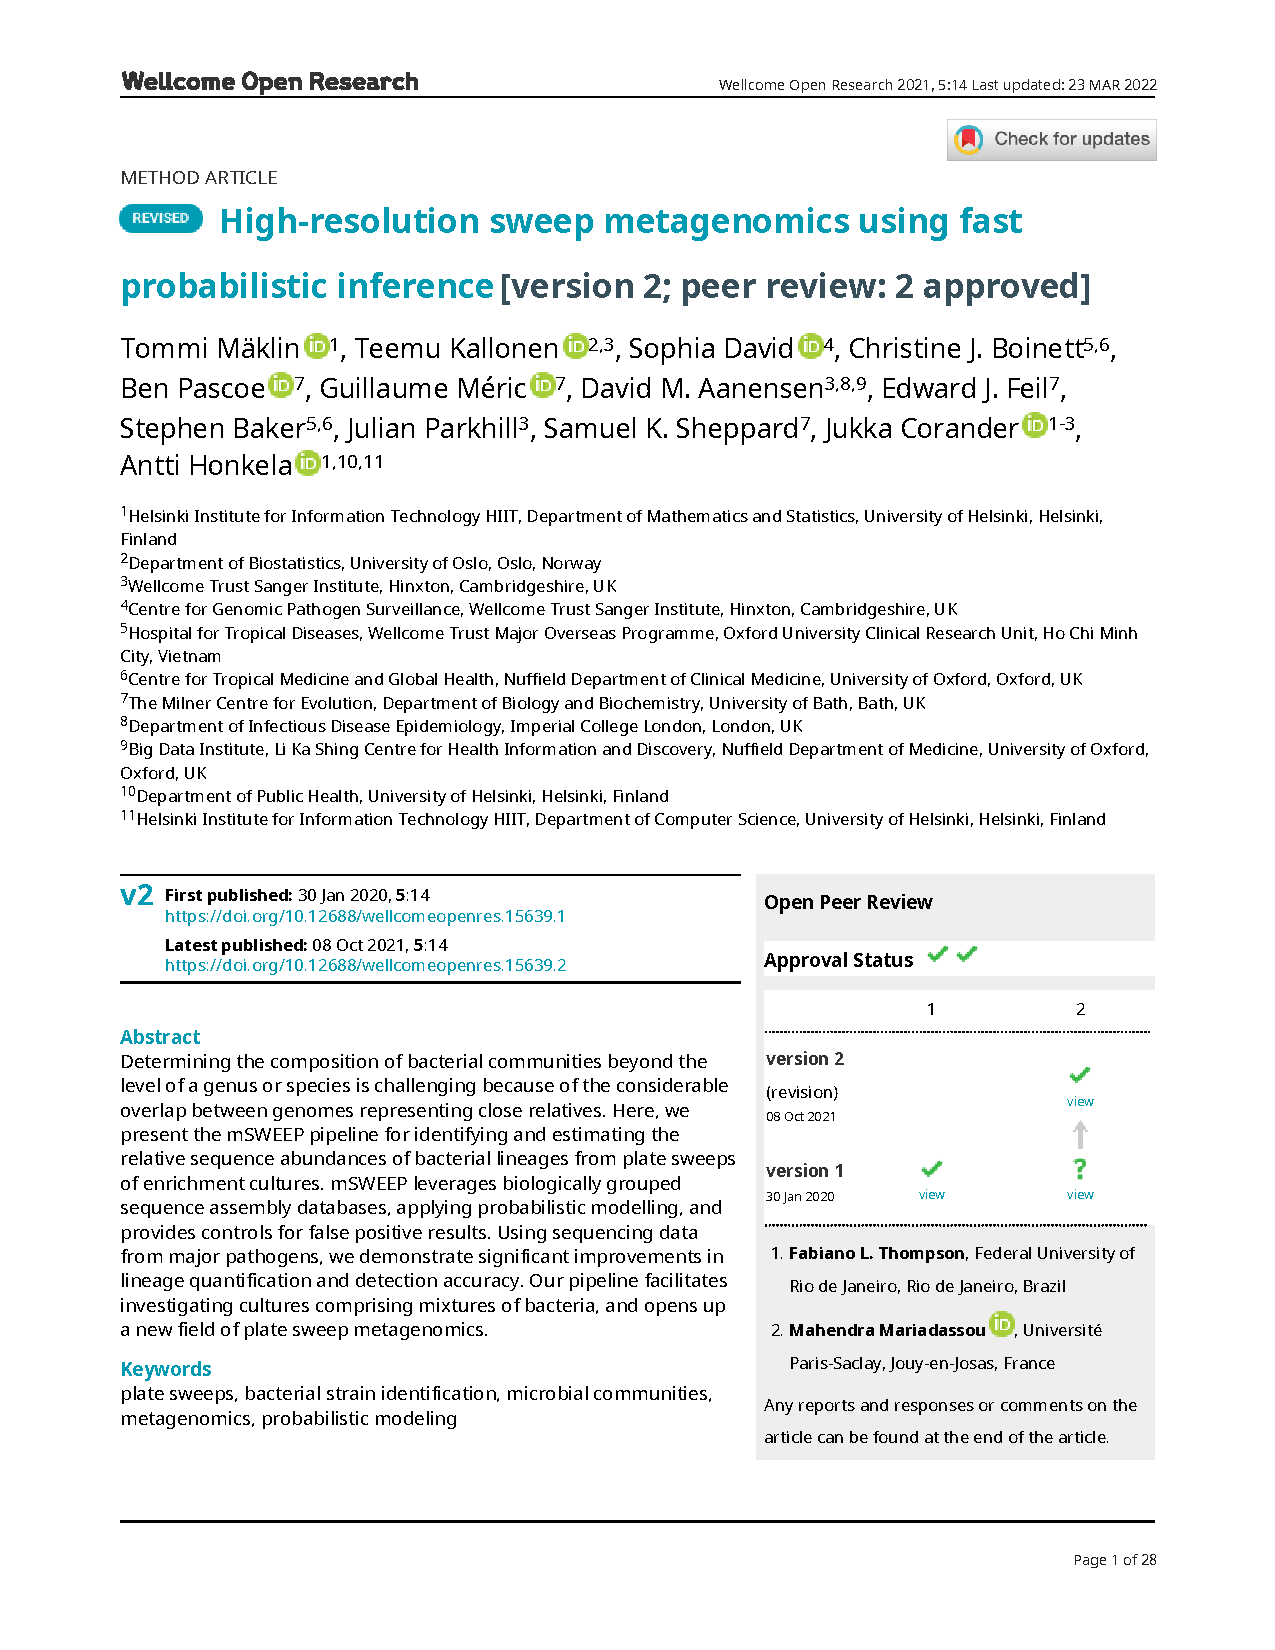
\includepdf[pages=-]{papers/maklin_high-resolution_2021.pdf}


% ******************************************************************************


\chapter*{Paper II}\thispagestyle{plain}
\addcontentsline{toc}{section}{Bacterial genomic epidemiology with mixed samples}

\note{I}{-222pt}{\dvWHITE}
%\notee{-222pt}{\dvWHITE}

\note{II}{-5pt}{black}
%\notee{-126.5pt}{\dvWHITE}

\note{III}{0pt}{\dvWHITE}
%\notee{-126.5pt}{\dvWHITE}

%% \note{IV}{-5pt}{\dvWHITE}
%% %\notee{-126.5pt}{\dvWHITE}

%% \note{V}{-5pt}{\dvWHITE}
%% %\notee{-126.5pt}{\dvWHITE}

%% \note{VI}{-5pt}{\dvWHITE}
%% %\notee{-126.5pt}{\dvWHITE}

\vspace{80pt}

% Here are the names of the authors
\underline{Tommi Mäklin}, Teemu Kallonen, Jarno Alanko, Ørjan
Samuelsen, Kristin Hegstad, Veli Mäkinen, Jukka Corander, Eva Heinz,
and Antti Honkela.

\vspace{10pt}
% Title of the 2nd paper
\noindent\textbf{Bacterial genomic epidemiology with mixed samples}

\vspace{10pt}
% Bibliographical information of the paper, for example, of a conference paper
\noindent In 
\emph{Microbial Genomics}, 
\\vol. 7 issue 11, 2021.

\vspace{60pt}
% Copyright information, for example, if the publisher is Springer
\noindent Copyright \textcopyright\ The Authors. This is an
open-access article distributed under the terms of the Creative
Commons Attribution License. This article was made open access via a
Publish and Read agreement between the Microbiology Society and the
corresponding author’s institution.

\cleardoublepage
% Including the original publication
\includepdf[pages=-]{papers/maklin_bacterial_2021.pdf}

% ******************************************************************************


\chapter*{Paper III}\thispagestyle{plain}
\addcontentsline{toc}{section}{Strong pathogen competition in neonatal gut colonization}

\note{I}{-222pt}{\dvWHITE}
%\notee{-222pt}{\dvWHITE}

\note{II}{-5pt}{\dvWHITE}
%\notee{-126.5pt}{\dvWHITE}

\note{III}{0pt}{black}
%\notee{-126.5pt}{\dvWHITE}

%% \note{IV}{-5pt}{\dvWHITE}
%% %\notee{-126.5pt}{\dvWHITE}

%% \note{V}{-5pt}{\dvWHITE}
%% %\notee{-126.5pt}{\dvWHITE}

%% \note{VI}{-5pt}{\dvWHITE}
%% %\notee{-126.5pt}{\dvWHITE}

\vspace{80pt}
% Here are the names of the authors
\underline{Tommi Mäklin}, Harry Thorpe, Anna Pöntinen, Rebecca Gladstone, Alan McNally, Ørjan
Samuelsen, Pål Johnsen, Trevor Lawley, Antti Honkela, and Jukka Corander.

\vspace{10pt}
% Title of the 3rd paper
\noindent\textbf{Strong pathogen competition in neonatal gut colonization}

\vspace{10pt}
% Bibliographical information of the paper, for example, a submitted paper
\noindent Submitted, preprint available from \emph{bioRxiv}.

\vspace{60pt}
%Copyright information, when the authors have the copyright of the paper
\noindent
The copyright holder for this preprint is the author/funder, who has
granted bioRxiv a license to display the preprint in perpetuity. It is
made available under a CC-BY 4.0 International license.

\cleardoublepage
% Including the original publication
%\includepdf[pages=-]{Publication_name_3.pdf}



% ******************************************************************************


%% \chapter*{Paper IV}\thispagestyle{empty}
%% \note{I}{-222pt}{\dvWHITE}
%% %\notee{-222pt}{\dvWHITE}

%% \note{II}{-100pt}{\dvWHITE}
%% %\notee{-126.5pt}{\dvWHITE}

%% \note{III}{-5pt}{\dvWHITE}
%% %\notee{-126.5pt}{\dvWHITE}

%% \note{IV}{-5pt}{black}
%% %\notee{-126.5pt}{\dvWHITE}

%% \note{V}{-5pt}{\dvWHITE}
%% %\notee{-126.5pt}{\dvWHITE}

%% \note{VI}{-5pt}{\dvWHITE}
%% %\notee{-126.5pt}{\dvWHITE}

%% \vspace{80pt}
%% % Here are the names of the authors
%% John Doe, Jane Doe, and John Smith

%% \vspace{10pt}
%% % Title of the 4th paper
%% \noindent\textbf{This is the title of the 4th paper}

%% \vspace{10pt}
%% % Bibliographical information of the paper, for example, of a journal paper
%% \noindent
%% In \emph{Journal name}, \\Volume xx, 20ZZ, pages XX-YY.

%% \vspace{60pt}
%% % Copyright information, when the authors have the copyright
%% \noindent Copyright \textcopyright\ The Authors.

%% \cleardoublepage
%% % Including the original publication
%% \includepdf[pages=-]{Publication_name_4.pdf}

% ******************************************************************************

\restoregeometry

%\end{document}


\end{document}
